\documentclass[11pt]{article}
\usepackage[utf8]{inputenc}
\usepackage[spanish]{babel}
\decimalpoint
\usepackage{amsmath}
\usepackage{amsthm}
\usepackage{amssymb}
\usepackage{graphicx}
\usepackage[margin=0.8in]{geometry}
\usepackage{fancyhdr}
\usepackage[inline]{enumitem}
\usepackage{float}
\usepackage{cancel}
\usepackage{bigints}
\usepackage{listings}
\usepackage{xcolor}
\usepackage{listingsutf8}
\usepackage{algpseudocode}
\usepackage{algorithm}
\usepackage{apacite}
\usepackage{tcolorbox}
\usepackage{multicol}
\usepackage{tipa}
\usepackage{caption} 
\pagestyle{fancy}
\usepackage{hyperref}
\usepackage{mathtools}% http://ctan.org/pkg/mathtools

\hypersetup{
    colorlinks,
    citecolor=black,
    filecolor=black,
    linkcolor=black,
    urlcolor=black
}
\newcommand{\xvdash}[1]{%
	\vdash^{\mkern-10mu\scriptscriptstyle\rule[-.9ex]{0pt}{0pt}#1}%
}
\setlength{\headheight}{15pt} 
\lhead{Tarea 3. Multiplicación de matrices distribuida utilizando paso de mensajes}
\rhead{\thepage}
\lfoot{ESCOM-IPN}
\renewcommand{\footrulewidth}{0.5pt}
\setlength{\parskip}{0.5em}
\newcommand{\ve}[1]{\overrightarrow{#1}}
\newcommand{\abs}[1]{\left\lvert #1 \right\lvert}
\newcommand{\blank}{\text{\textcrb}}
\date{\today}
\title{Tarea 3. Multiplicación de matrices distribuida utilizando paso de mensajes}
\author{Sanchez Mendez Edmundo Josue}

\lstset{
tabsize = 4, %% set tab space width
showstringspaces = false, %% prevent space marking in strings, string is defined as the text that is generally printed directly to the console
numbers = left, %% display line numbers on the left
commentstyle = \color{green}, %% set comment color
keywordstyle = \color{blue}, %% set keyword color
stringstyle = \color{red}, %% set string color
rulecolor = \color{black}, %% set frame color to avoid being affected by text color
basicstyle = \small \ttfamily , %% set listing font and size
breaklines = true, %% enable line breaking
numberstyle = \tiny,
}

\bibliographystyle{apacite}
\begin{document}
		\begin{titlepage}
			\begin{center}
				
				% Upper part of the page. The '~' is needed because \\
				% only works if a paragraph has started.
				
				\noindent
				\begin{minipage}{0.5\textwidth}
					\begin{flushleft} \large
						
\includegraphics[width=0.5\textwidth]{resources/ipn.png}
					\end{flushleft}
				\end{minipage}%
				\begin{minipage}{0.55\textwidth}
					\begin{flushright} \large
						
\includegraphics[width=0.5\textwidth]{resources/escom.png}
					\end{flushright}
				\end{minipage}
				
				\textsc{\LARGE Instituto Politécnico Nacional}\\[0.5cm]
				
				\textsc{\Large Escuela Superior de Cómputo}\\[1cm]
				
				% Title
				
				{ \huge Tarea 3. Multiplicación de matrices distribuida utilizando paso de mensajes  \\[1cm] }
				
				{ \Large Unidad de aprendizaje: Desarrollo de Sistemas Distribuidos} \\[1cm]
				
				{ \Large Grupo: 4CV11 } \\[1cm]
				
				\noindent
				\begin{minipage}{0.5\textwidth}
					\begin{flushleft} \large
						\emph{Alumno:} \\
						Sanchez Mendez Edmundo Josue
					\end{flushleft}
				\end{minipage}%
				\begin{minipage}{0.5\textwidth}
					\begin{flushright} \large
						\emph{Profesor:} \\
						Pineda Guerrero Carlos 
					\end{flushright}
				\end{minipage}
				
				\vfill
				% Bottom of the page
				{\large {\today}}
			\end{center}
		\end{titlepage}
	
	\titlepage
	\tableofcontents
	\newpage
	
	\section{Introducción}
		Mediante el desarrollo de un sistema distribuido el cual tendrá una topología lógica de estrella en donde interceden 5 nodos, en el cual el nodo 0 sera el nodo central de la topología, el objetivo de la practica es llevar acabo una multiplicación de matrices de tamaño N, para esta practica N sera igual a 10 y a 1500.\par
		El funcionamiento del programa es el siguiente:
		\begin{itemize}
			\item Se tendrán 3 matrices, A, B y C de tipo long y tamaño $NxN$.
			\item El nodo 0 sera el encargado de realizar lo siguiente: 
				\begin{itemize}
					\item Inicializar las matrices A y B con los siguientes valores: A[i][j]=$i+2*j$ y B[i][j]=$i-2*j$.
					\item Transponer la matriz B.
					\item Enviar la matriz A1 al nodo 1.
					\item Enviar la matriz B1 al nodo 1.
					\item Enviar la matriz A1 al nodo 2.
					\item Enviar la matriz B2 al nodo 2.
					\item Enviar la matriz A2 al nodo 3.
					\item Enviar la matriz B1 al nodo 3.
					\item Enviar la matriz A2 al nodo 4.
					\item Enviar la matriz B2 al nodo 4.
					\item Recibir la matriz C1 del nodo 1.
					\item Recibir la matriz C2 del nodo 2.
					\item Recibir la matriz C3 del nodo 3.
					\item Recibir la matriz C4 del nodo 4.
					\item Calcular el checksum de la matriz C, con base a la siguiente formula: \[ \sum_{i=0,j=0}^{N-1}C[i][j] 
\].
					\item Desplegar el checksum de la matriz C.
					\item Si N=10 entonces desplegar las matrices A, B y C
				\end{itemize}				
			\item El nodo 1 sera el encargado de realizar lo siguiente.
				\begin{itemize}
					\item Recibir del nodo 0 la matriz A1.
					\item Recibir del nodo 0 la matriz B1.
					\item Realizar el producto C1=A1xB1 (renglón por renglón).
					\item Enviar la matriz C1 al nodo 0.
				\end{itemize}	
			\item El nodo 2 sera el encargado de realizar lo siguiente.
				\begin{itemize}
					\item Recibir del nodo 0 la matriz A1.
					\item Recibir del nodo 0 la matriz B2.
					\item Realizar el producto C2=A1xB2 (renglón por renglón).
					\item Enviar la matriz C2 al nodo 0.
				\end{itemize}
			\item El nodo 3 sera el encargado de realizar lo siguiente.
				\begin{itemize}
					\item Recibir del nodo 0 la matriz A2.
					\item Recibir del nodo 0 la matriz B1.
					\item Realizar el producto C3=A2xB1 (renglón por renglón).
					\item Enviar la matriz C3 al nodo 0.
				\end{itemize}
			\item El nodo 4 sera el encargado de realizar lo siguiente.
				\begin{itemize}
					\item Recibir del nodo 0 la matriz A2.
					\item Recibir del nodo 0 la matriz B2.
					\item Realizar el producto C4=A2xB2 (renglón por renglón).
					\item Enviar la matriz C4 al nodo 0.
				\end{itemize}
		\end{itemize}
	\section{Desarrollo}
Para poder desarrollar esta tarea se tomo como ejemplo la tarea 1 y el código enseñado en clase de multiplicación de matrices, basándonos en el archivo MultiplicaMatriz\_ 2.java. Una vez programado el sistema distribuido con base en los requerimientos solicitados para la tarea se procede a crear las 5 maquinas virtuales en Azure para el cumplimiento de el tipo de topologia que estamos usando. En las figuras de la 1 a la 7 se ve la creación del nodo 0 como maquina virtual en Azure cumpliendo con las características señaladas en la tarea la cual se nos pide que el OS sea Ubuntu con 1 CPU, 1GB de RAM y disco HDD estándar, ademas de llevar como nombre M2019630428-n, donde n es el número de nodo.
		\begin{figure}[H]
			\centering
			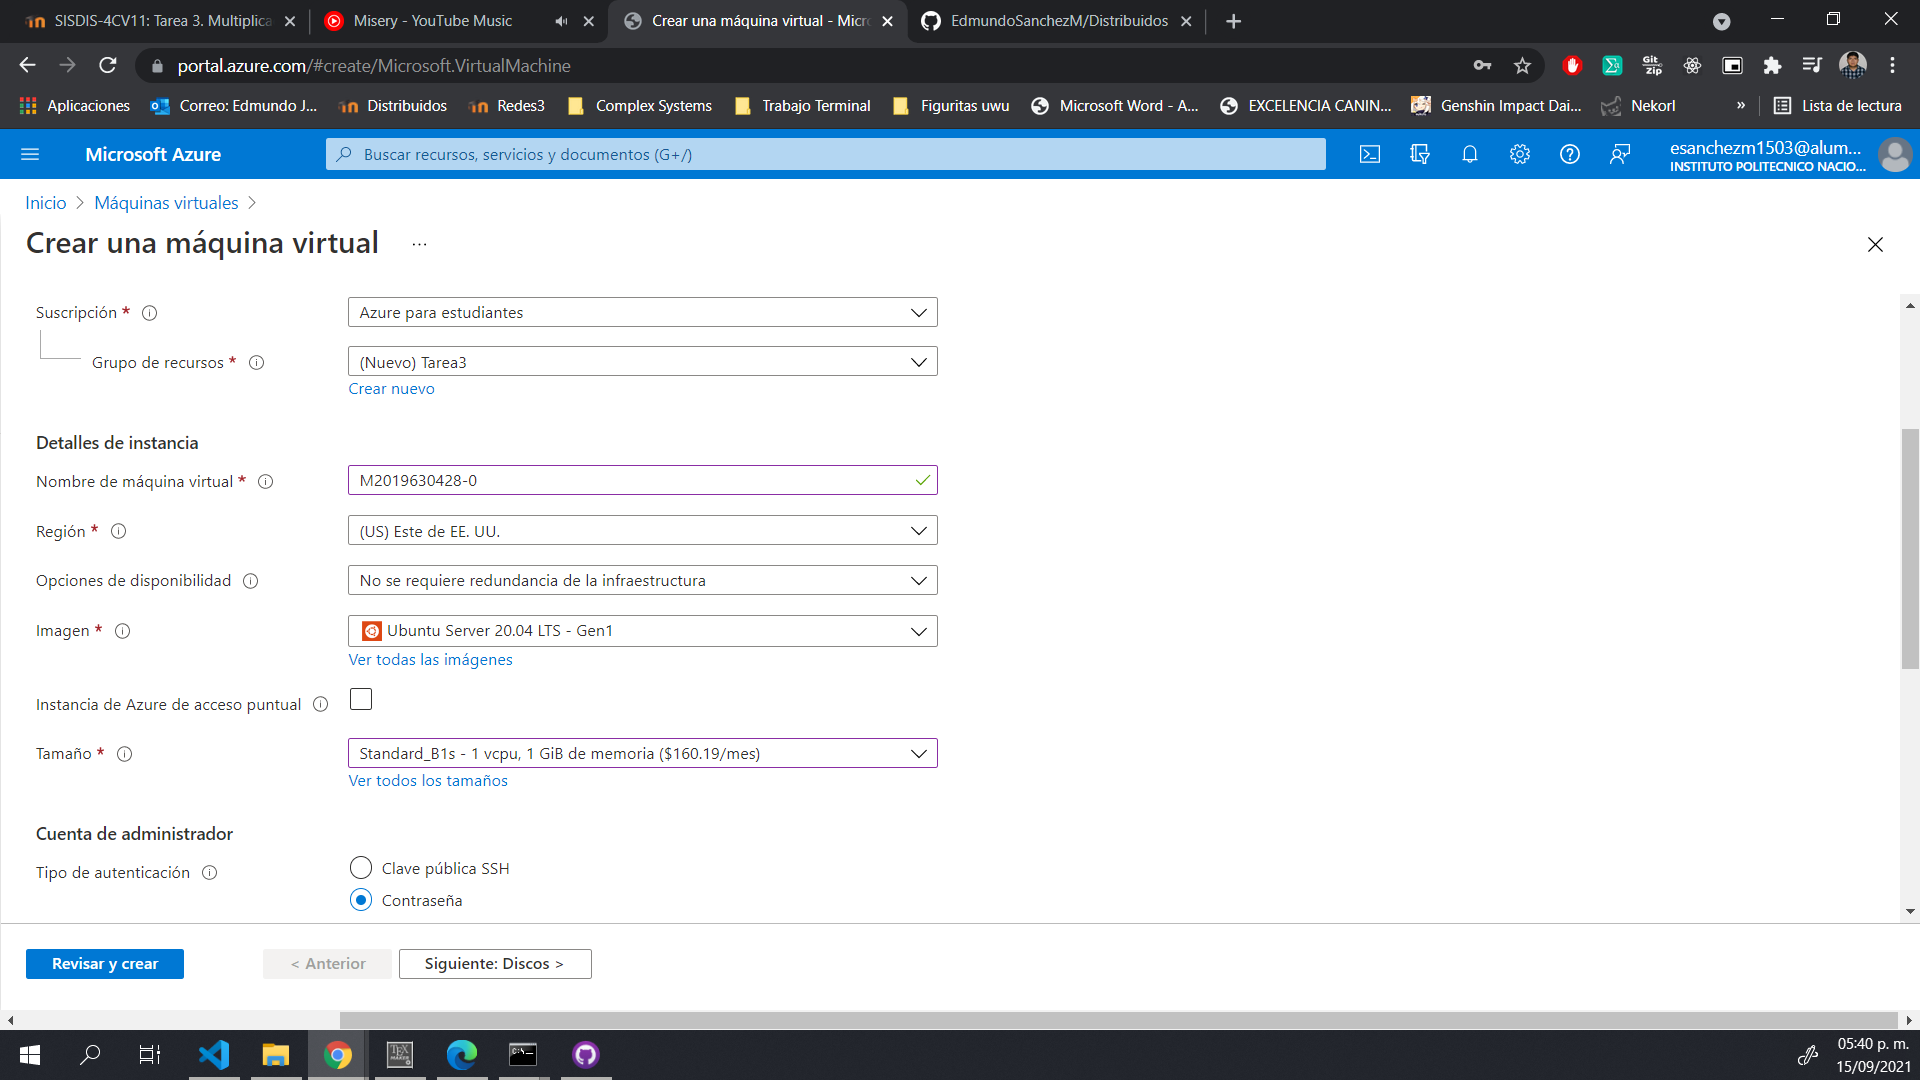
\includegraphics[scale=0.34]{resources/datosbasicos.png}
			\caption{Datos básicos para el nodo 0. }\label{fig:picture}
		\end{figure}
		\begin{figure}[H]
			\centering
			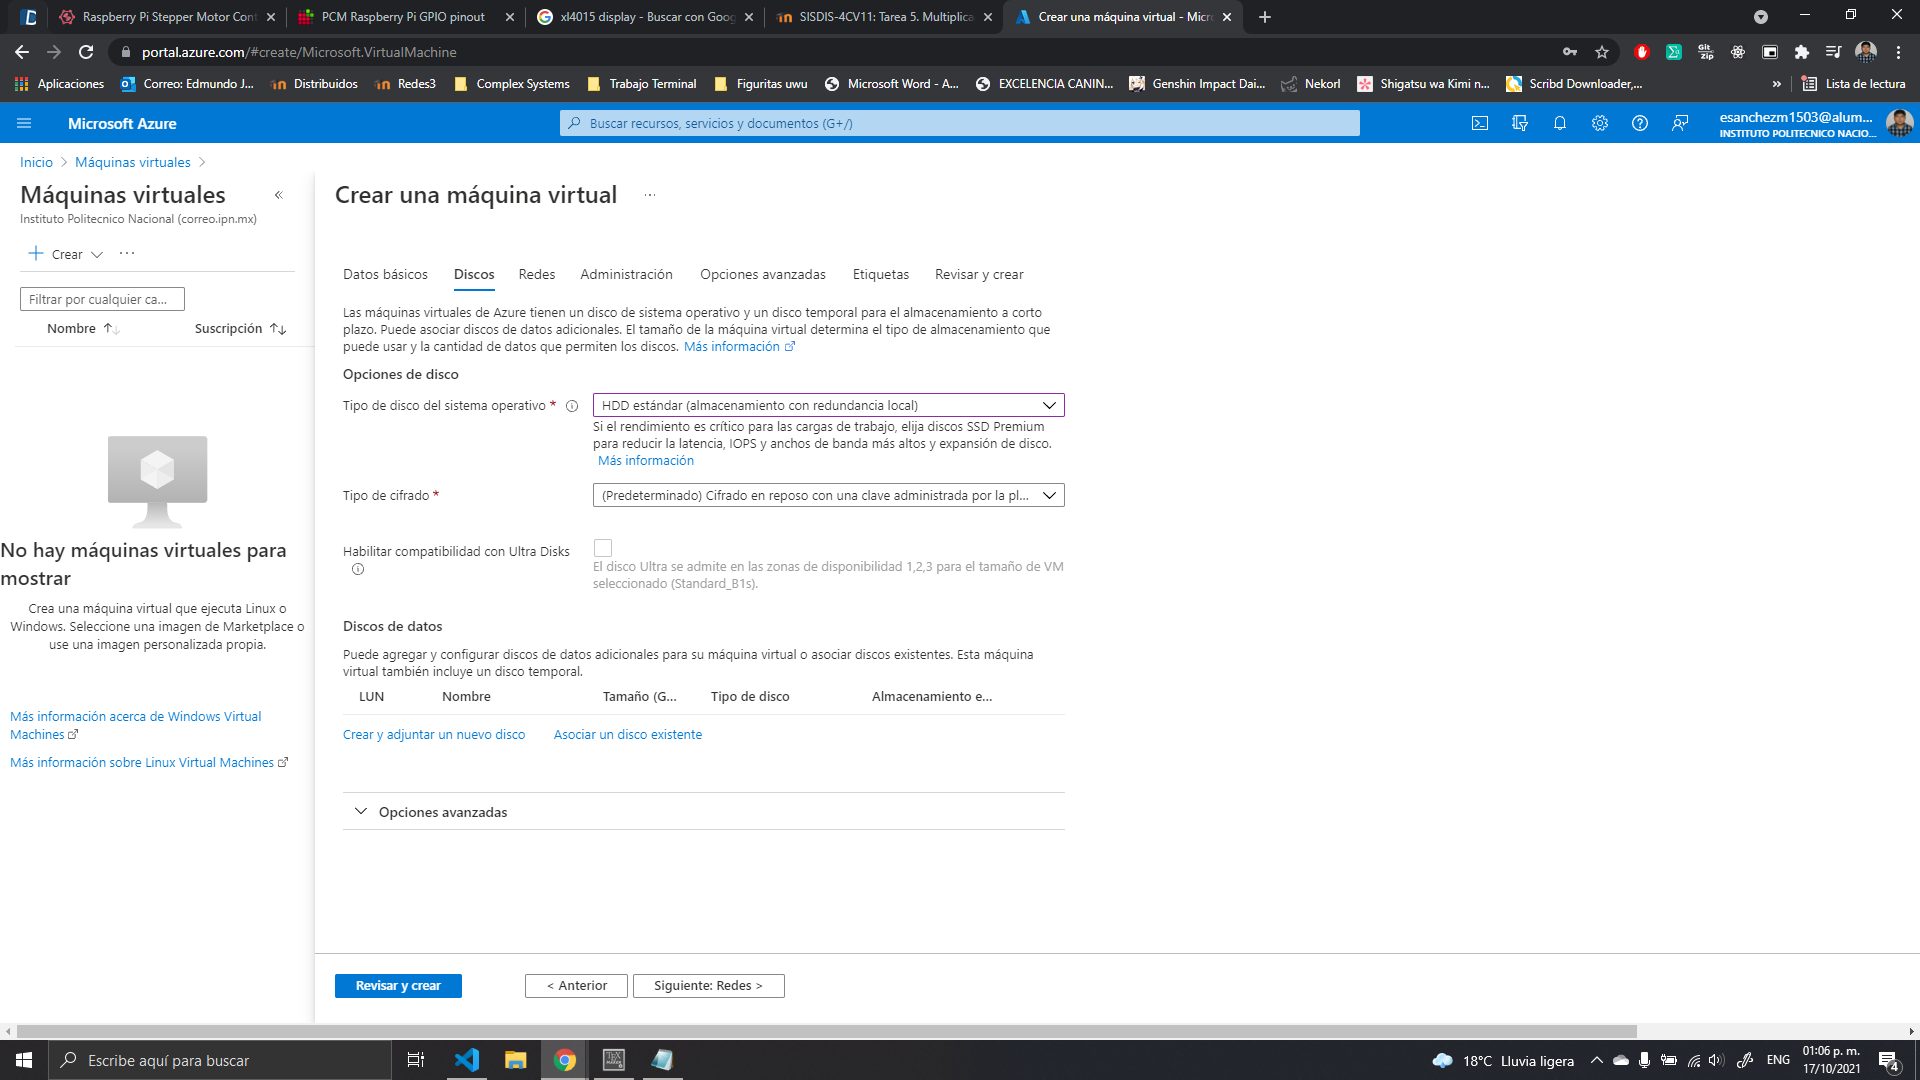
\includegraphics[scale=0.34]{resources/datosdisco.png}
			\caption{Configuración del tipo de disco para el nodo 0. }\label{fig:picture}
		\end{figure}
		\begin{figure}[H]
			\centering
			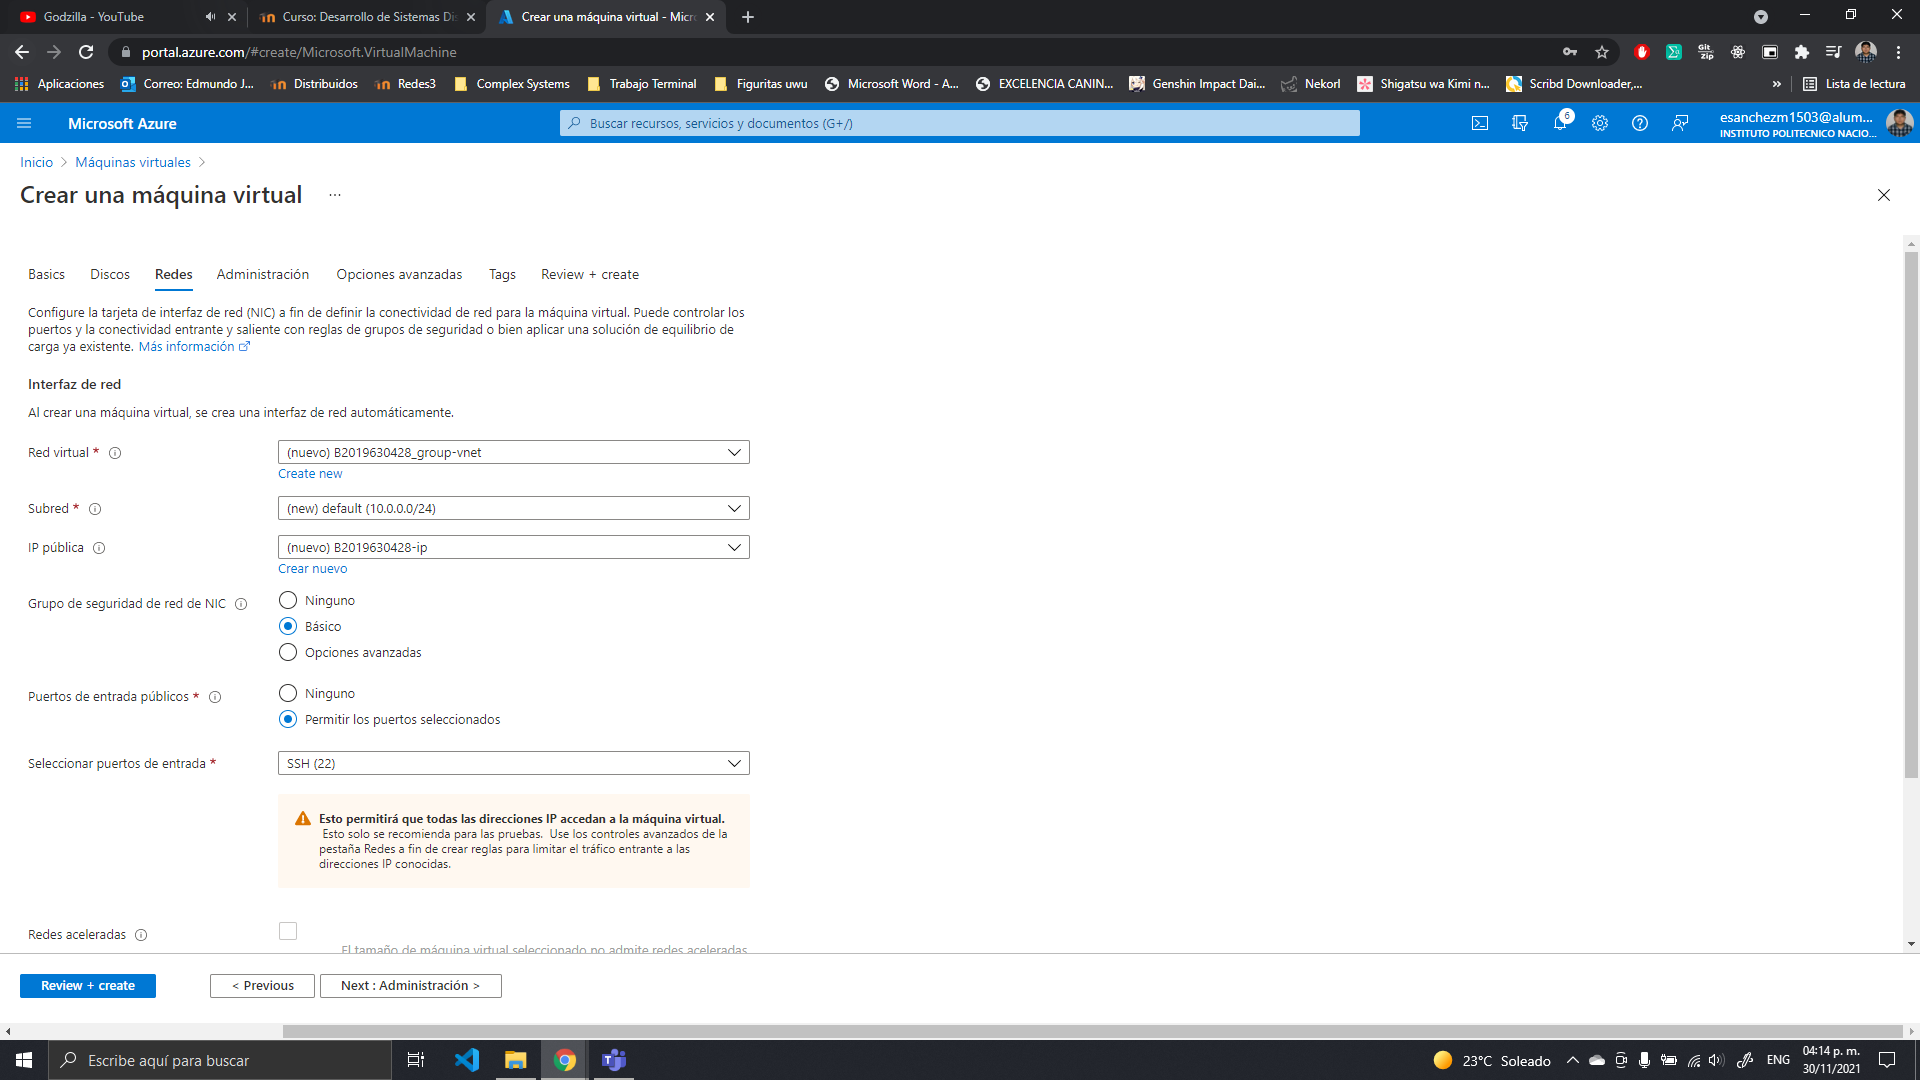
\includegraphics[scale=0.34]{resources/datosredes.png}
			\caption{Información sobre la redes para el nodo 0. }\label{fig:picture}
		\end{figure}
		\begin{figure}[H]
			\centering
			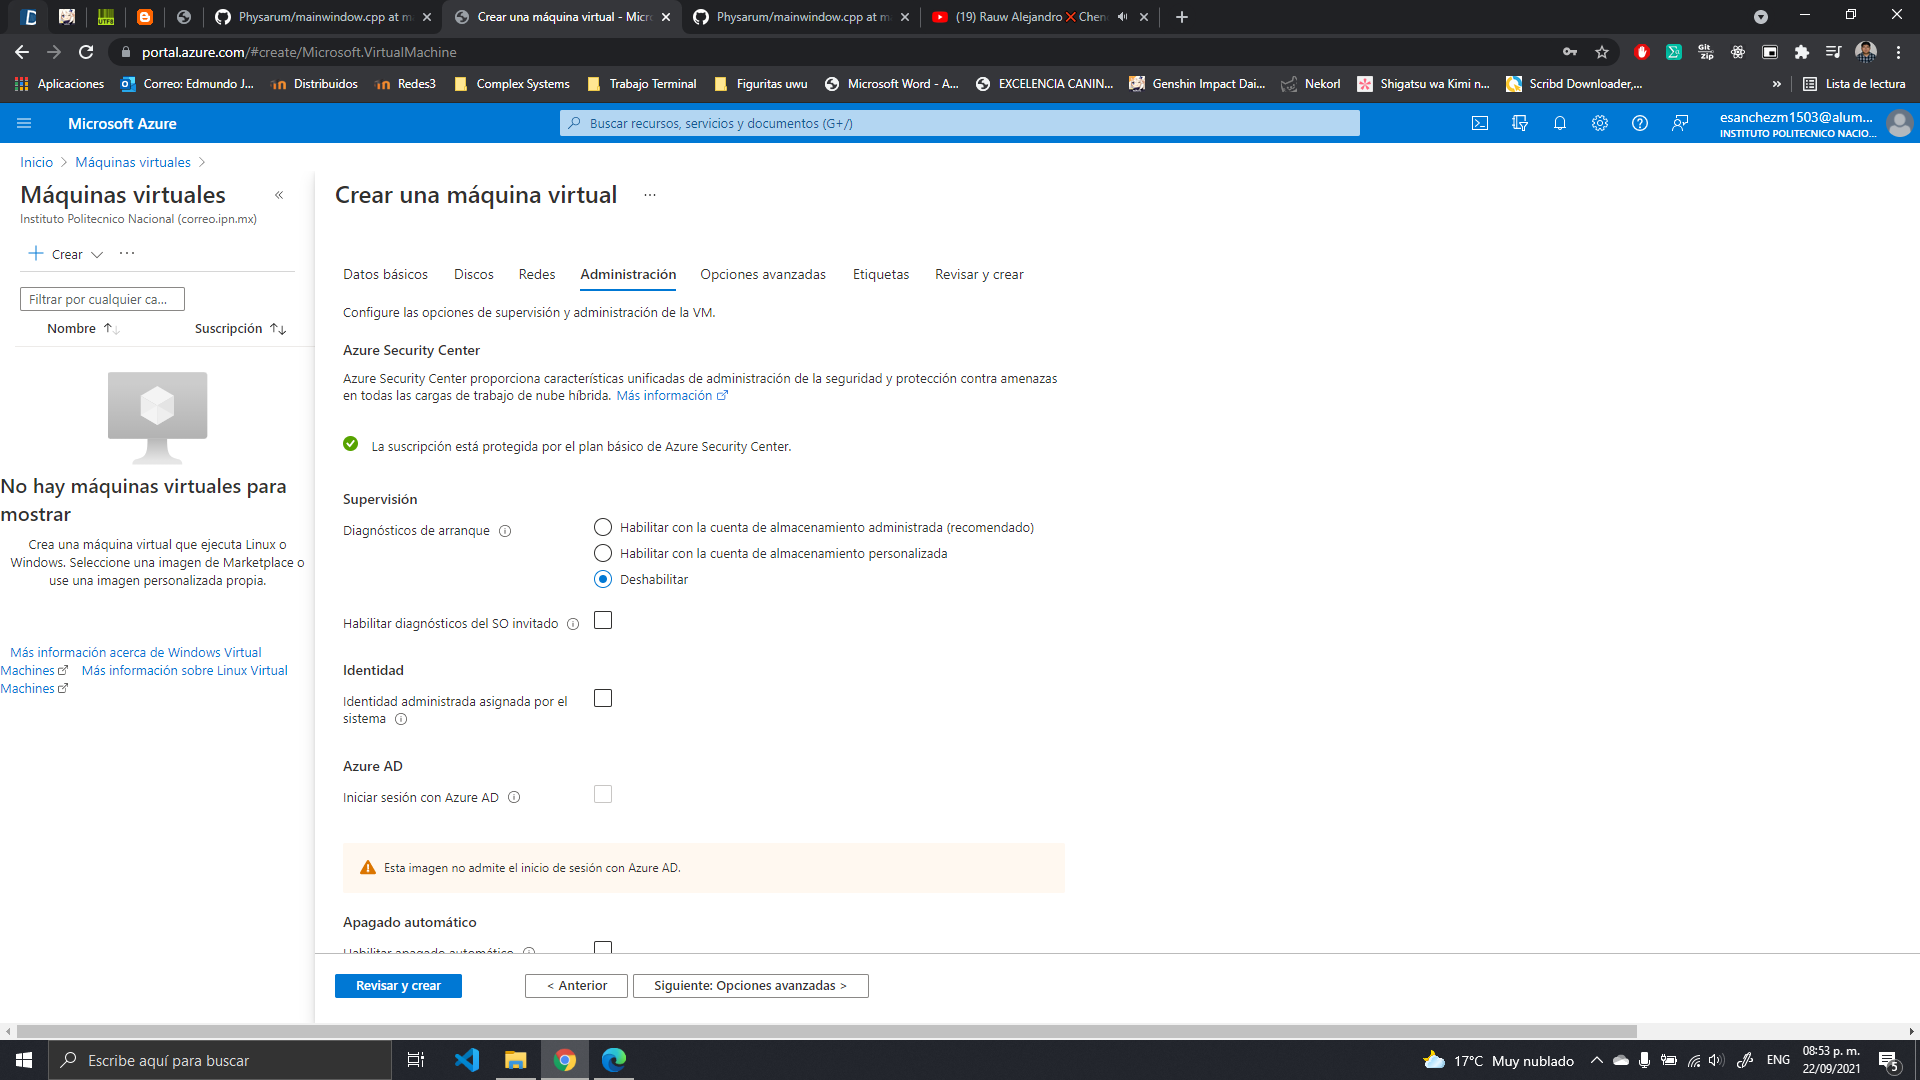
\includegraphics[scale=0.34]{resources/datosadministracion.png}
			\caption{Configuración de la administración para el nodo 0. }\label{fig:picture}
		\end{figure}
		\begin{figure}[H]
			\centering
			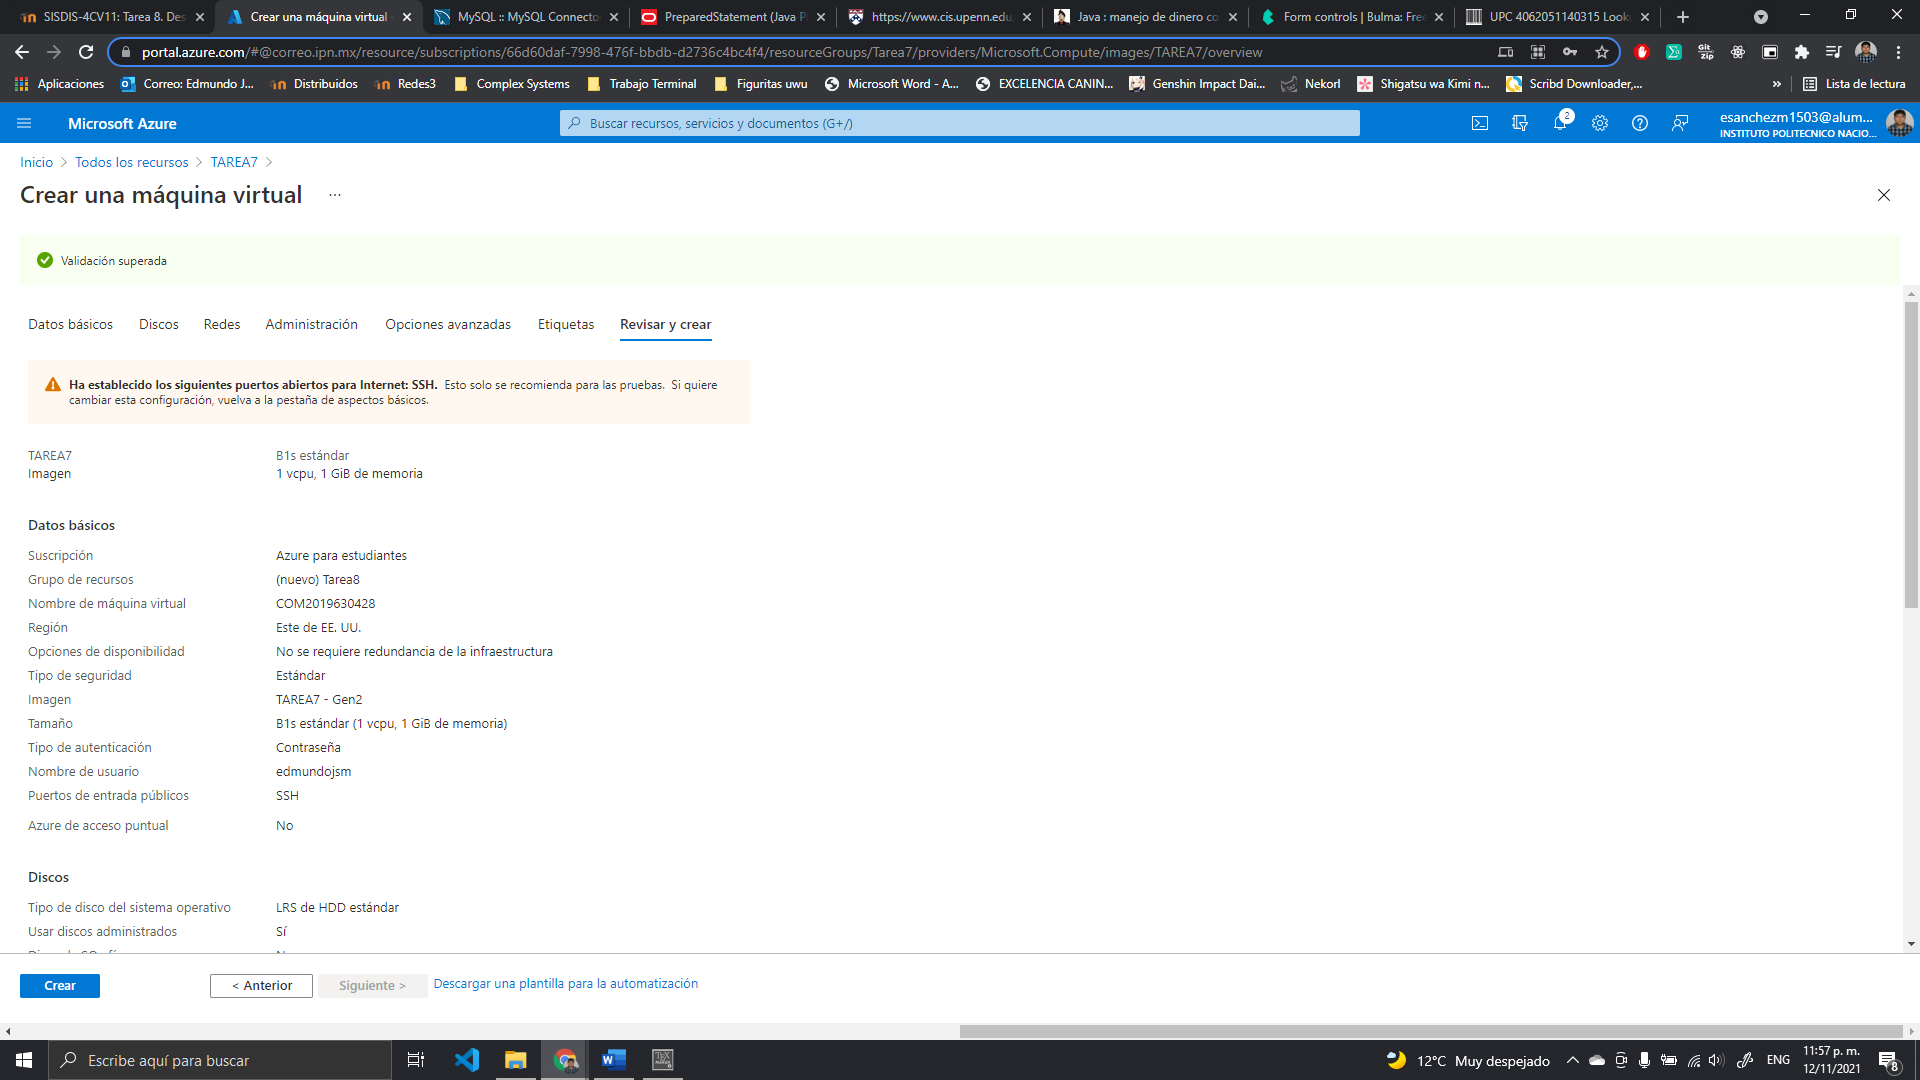
\includegraphics[scale=0.34]{resources/revisarycrear.png}
			\caption{Creación de la maquina virtual para el nodo 0. }\label{fig:picture}
		\end{figure}
		\begin{figure}[H]
			\centering
			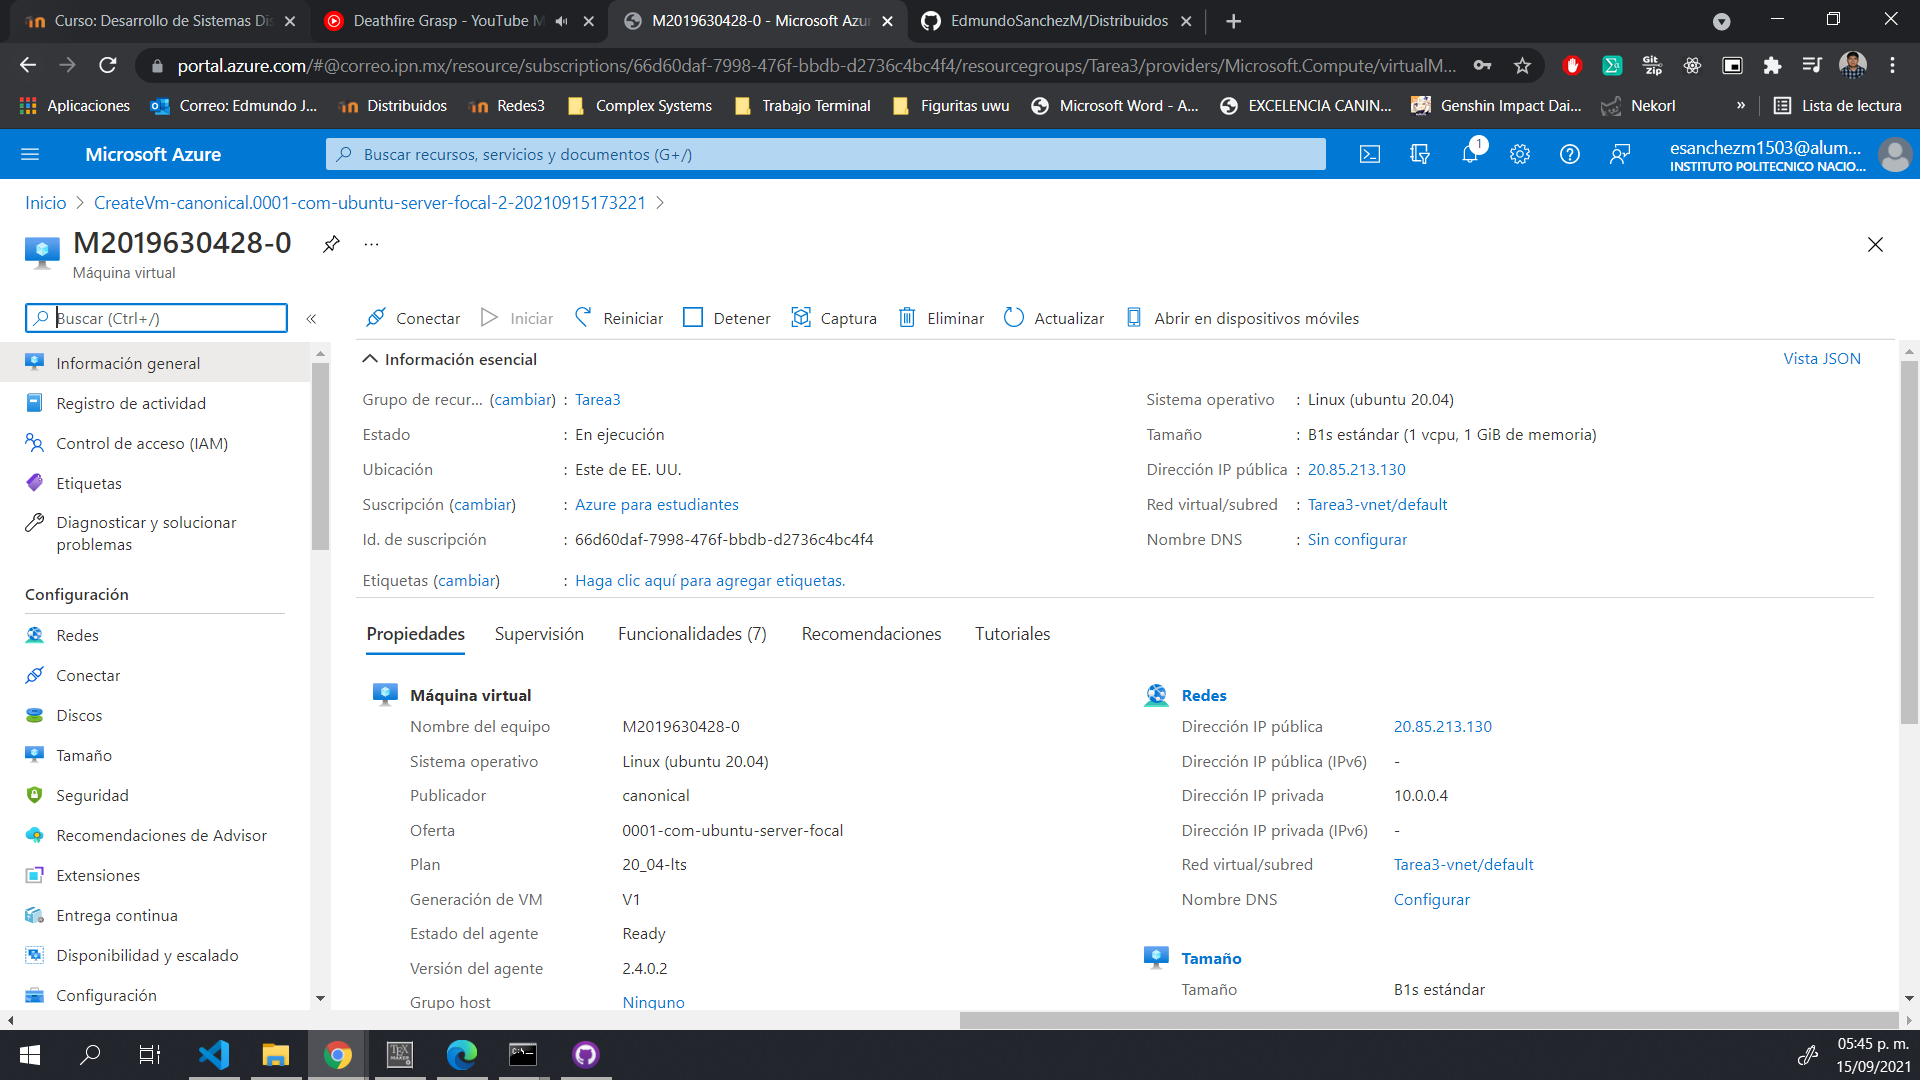
\includegraphics[scale=0.34]{resources/Panelcontrol.png}
			\caption{Panel de control de la maquina virtual para el nodo 0. }\label{fig:picture}
		\end{figure}
		\begin{figure}[H]
			\centering
			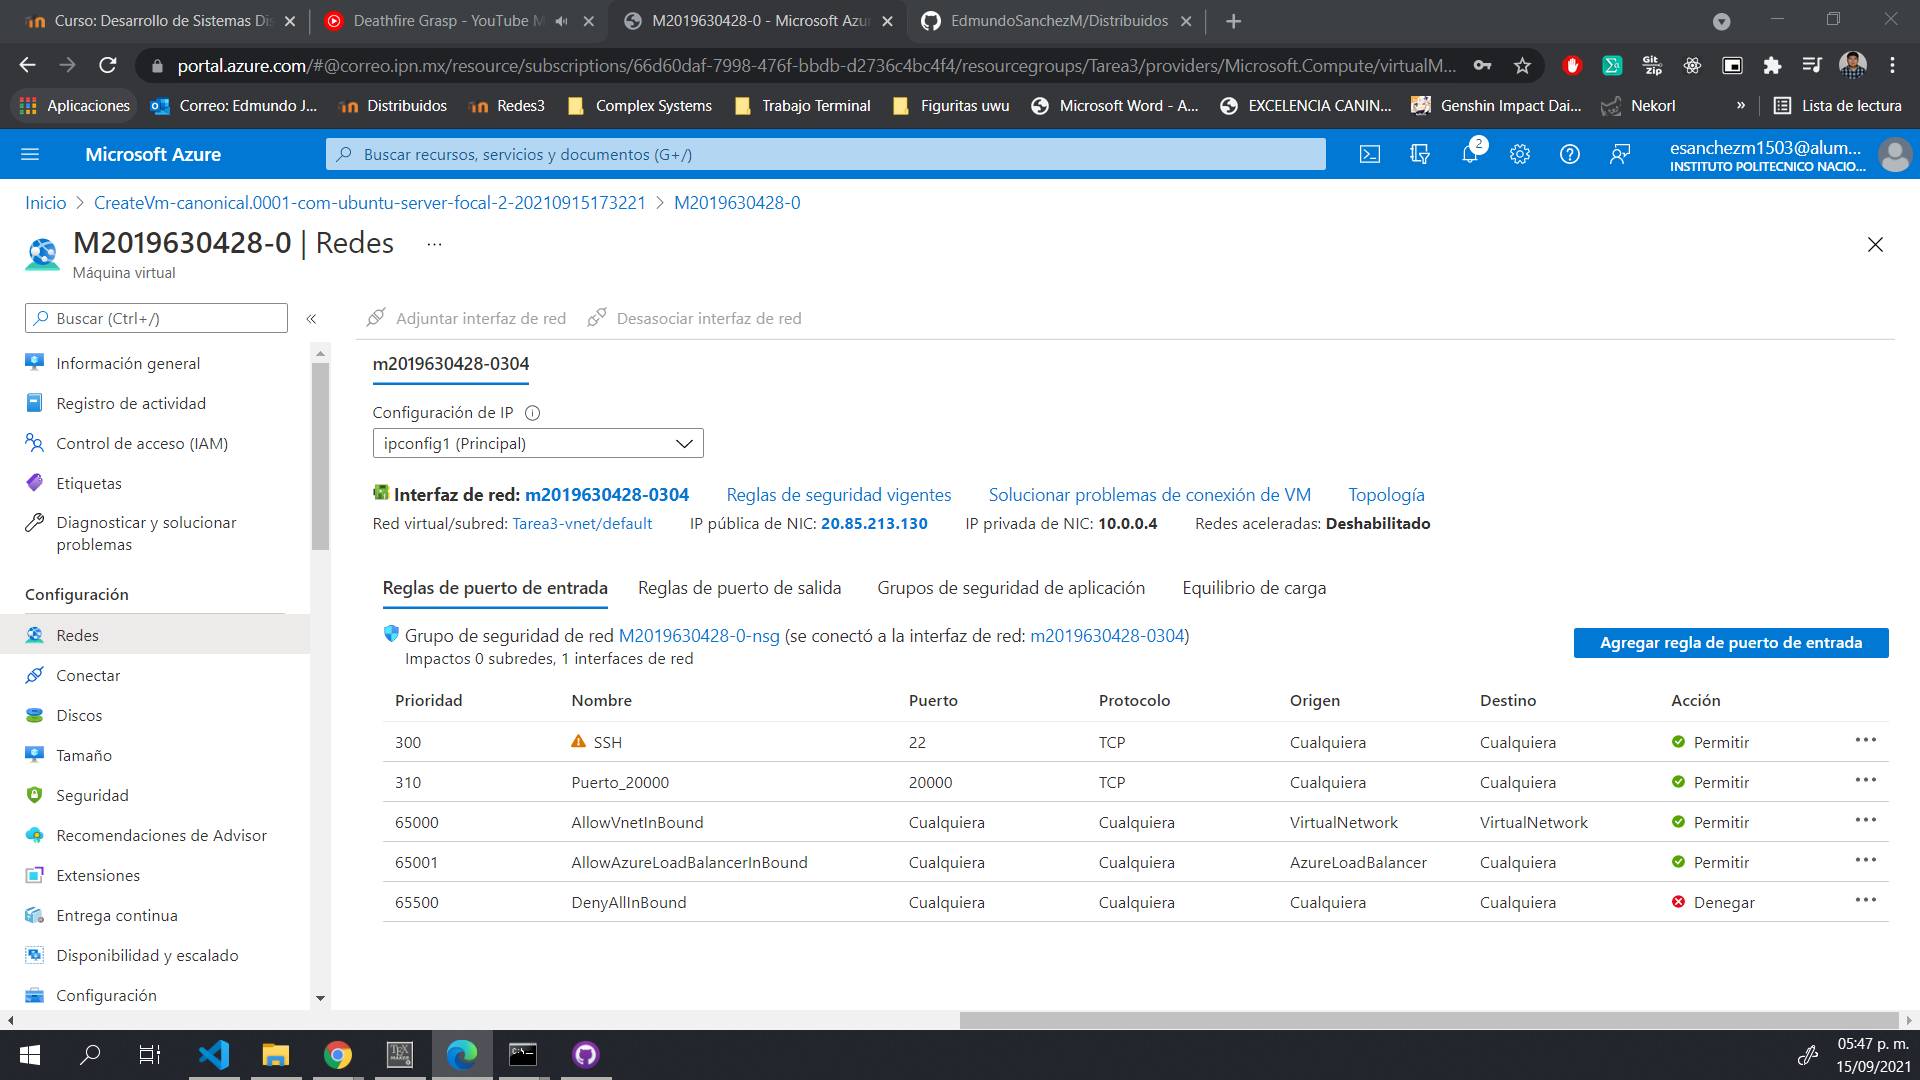
\includegraphics[scale=0.34]{resources/puerto20000abierto.png}
			\caption{Apertura del puerto 20000 en el nodo 0. }\label{fig:picture}
		\end{figure}
Las imágenes de la 1 a la 7 se tuvieron que repetir cuatro veces mas, esto debido al tipo de topologia a implementar, mencionar que en mi caso al momento de querer crear una quinta maquina virtual con las características dadas en la tarea no se me dejo, ya que tengo un limite de 4 maquinas al usar standar\_ B1, por lo que tuve que crear una maquina virtual con otras características, intente aumentar el limite que tengo pero no me fue posible ya que me solicitan crear un token con el soporte técnico, sin embargo, al usar una maquina con otras características aparentemente no me genero un gran costo como pensaba que seria.\par
Una vez creadas las maquinas virtuales se procedió a hacer lo que se muestra en las figuras de 8 y 9 por las 5 maquinas que tenemos, usamos como ejemplo el nodo 0
		\begin{figure}[H]
			\centering
			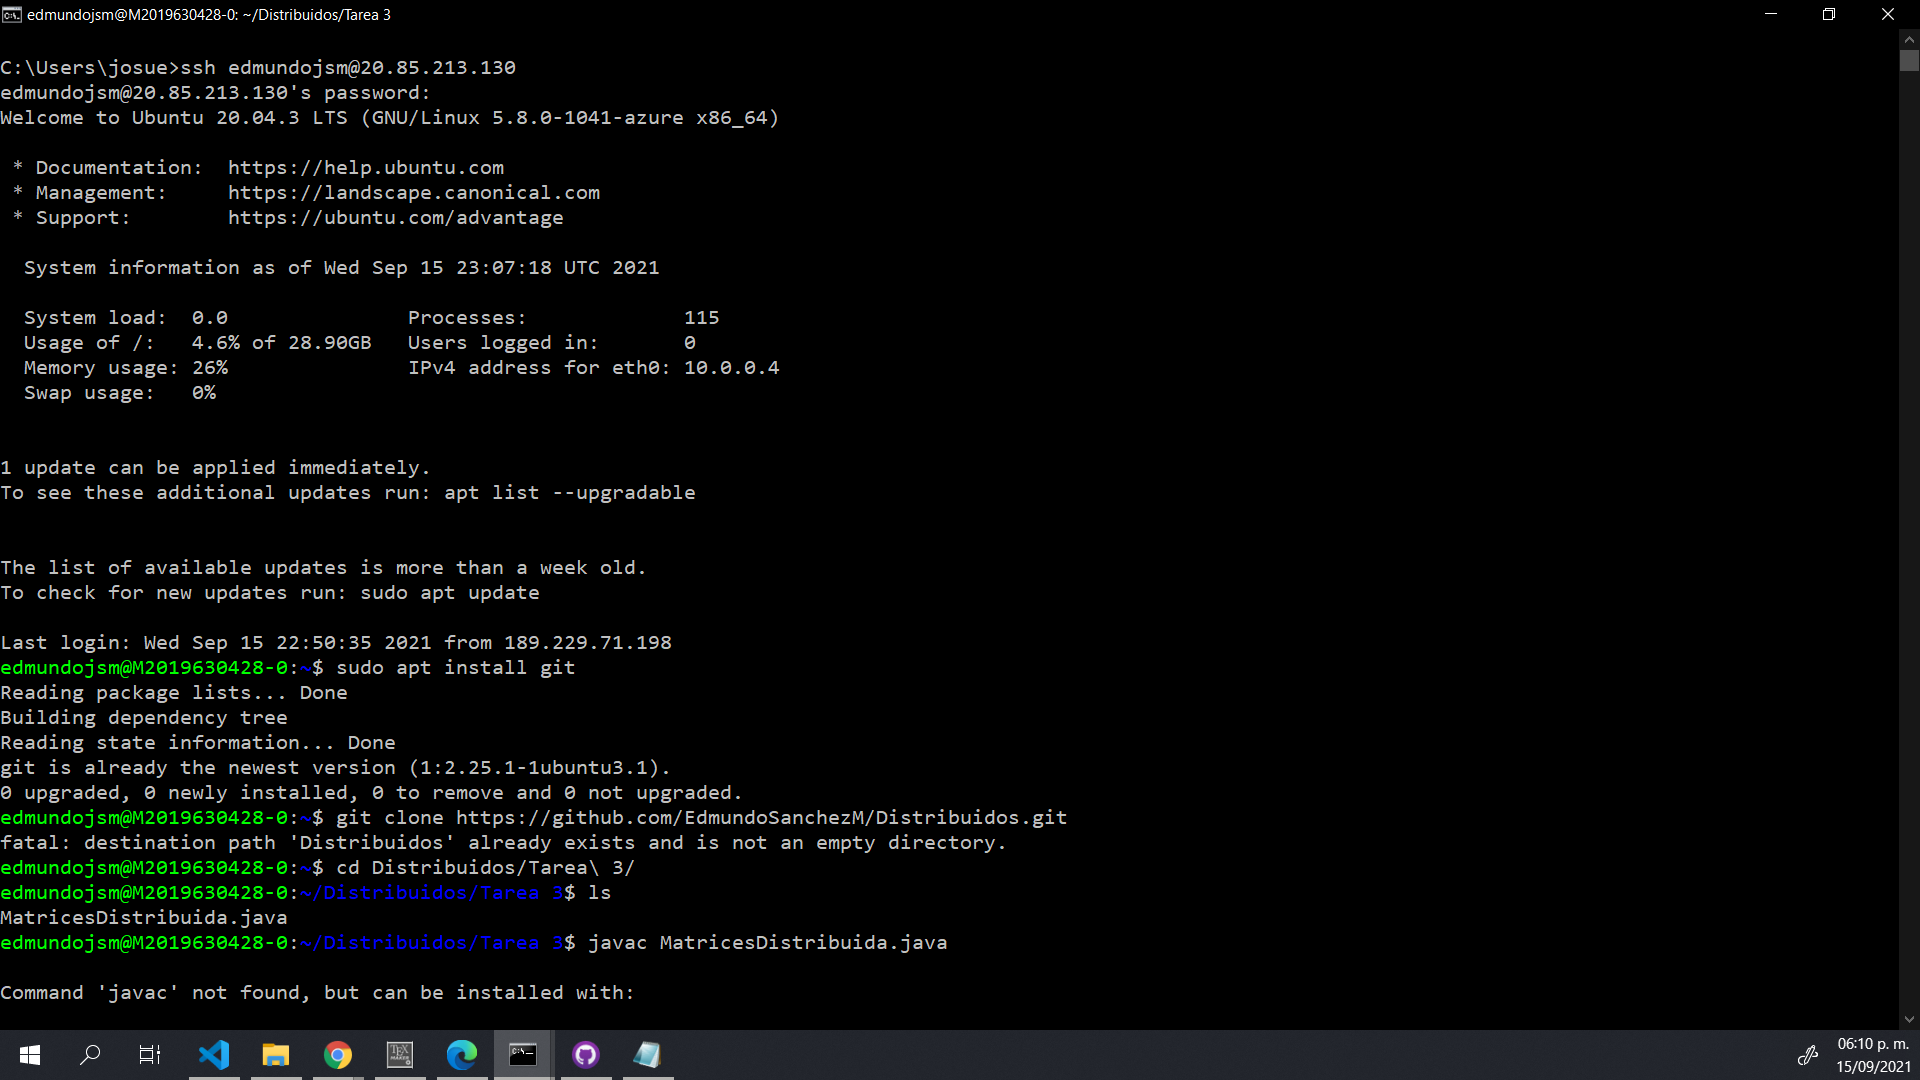
\includegraphics[scale=0.34]{resources/Nodo0ssh.png}
			\caption{Conexión vía ssh a la maquina virtual que hará como nodo 0. }\label{fig:picture}
		\end{figure}
		\begin{figure}[H]
			\centering
			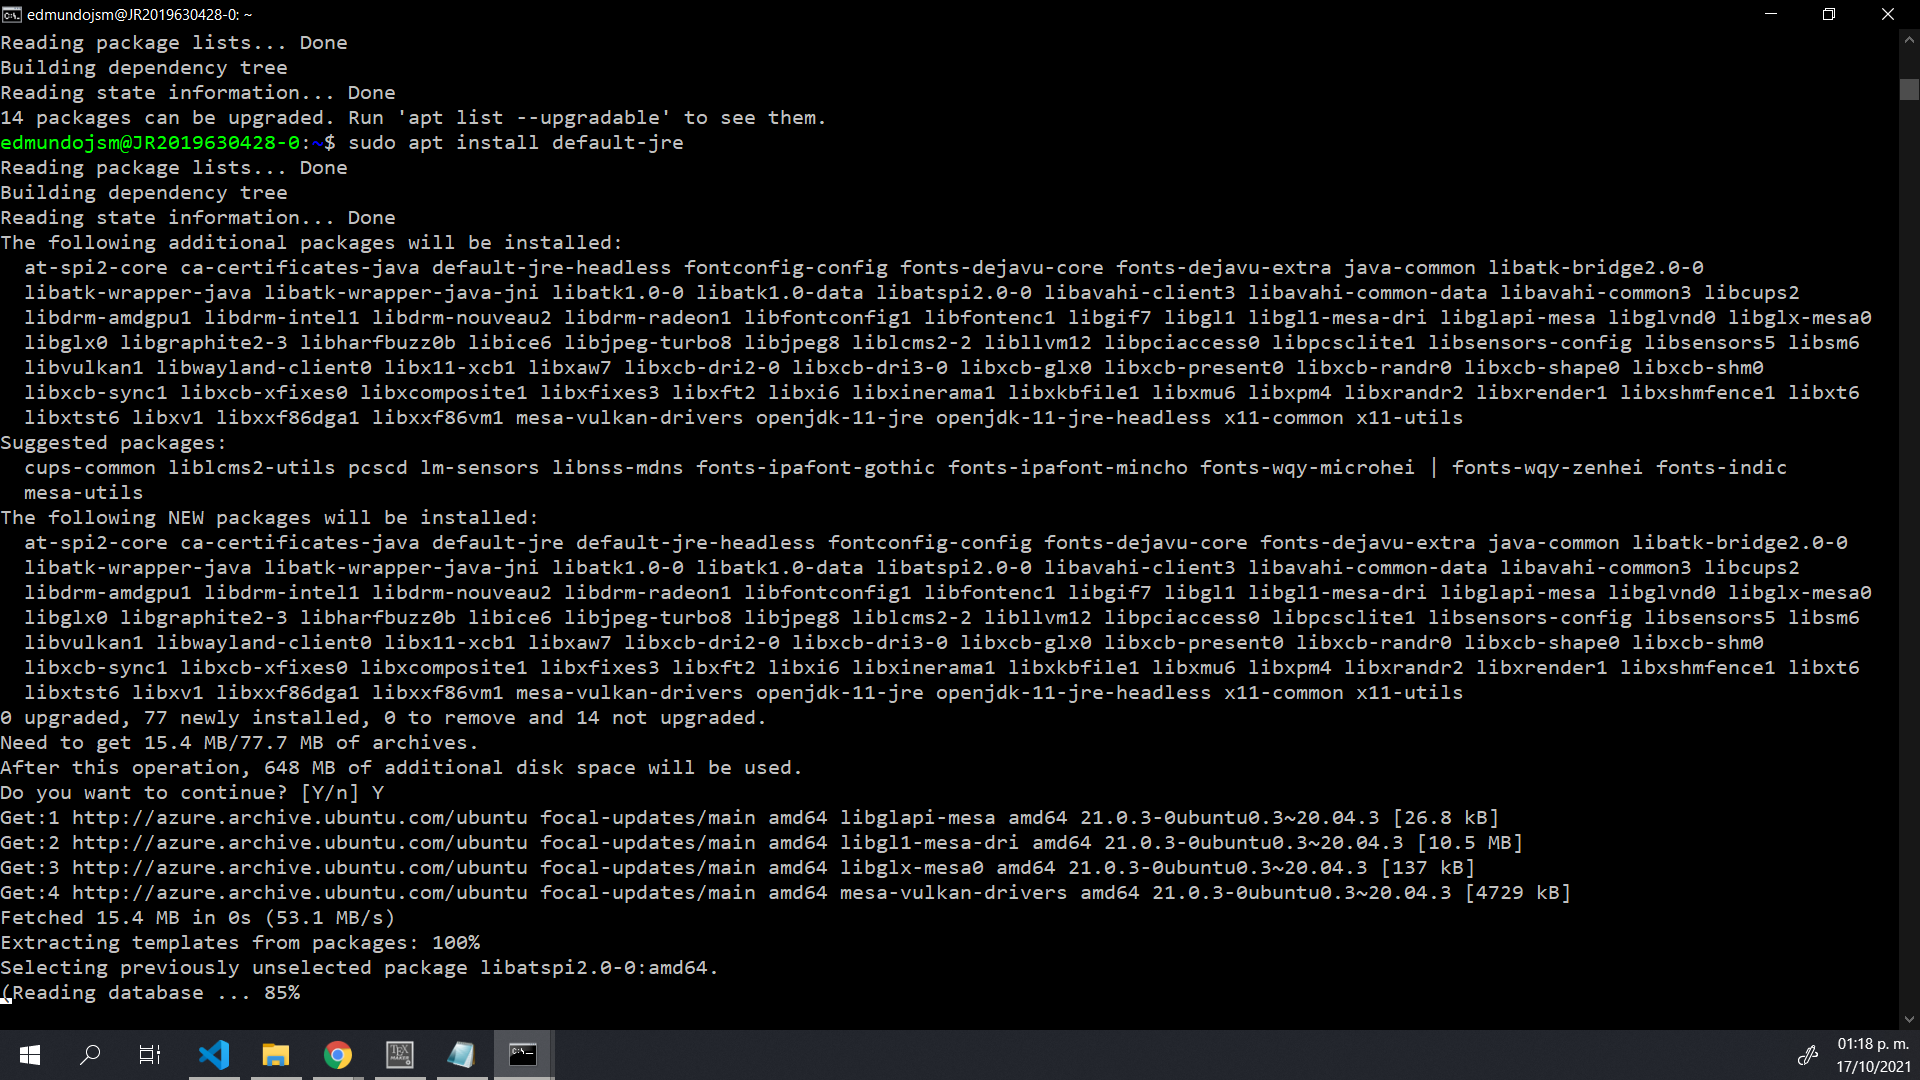
\includegraphics[scale=0.34]{resources/instalarjava.png}
			\caption{Instalación del jdk en el nodo 0. }\label{fig:picture}
		\end{figure}
		Una vez configurado cada maquina virtual se procedió a clonar un repositorio privado de mi autoría almacenado en GitHub, esto para poder compartir el archivo necesario para el funcionamiento de la practica, esto se puede ver en la figura 11. Una vez de tener configurada la maquina virtual y teniendo el archivo necesario para el cumplimiento de la tarea se procede a la siguiente fase de la tarea, la compilación del código.
		\subsection{Compilación del código}
		En la figura 10 podemos ver como la compilación de nuestro programa MatricesDistribuida.java se hace de manera exitosa y sin ningún error alguno, esto desde la terminal de Ubuntu de nuestra maquina virtual.
		\begin{figure}[H]
			\centering
			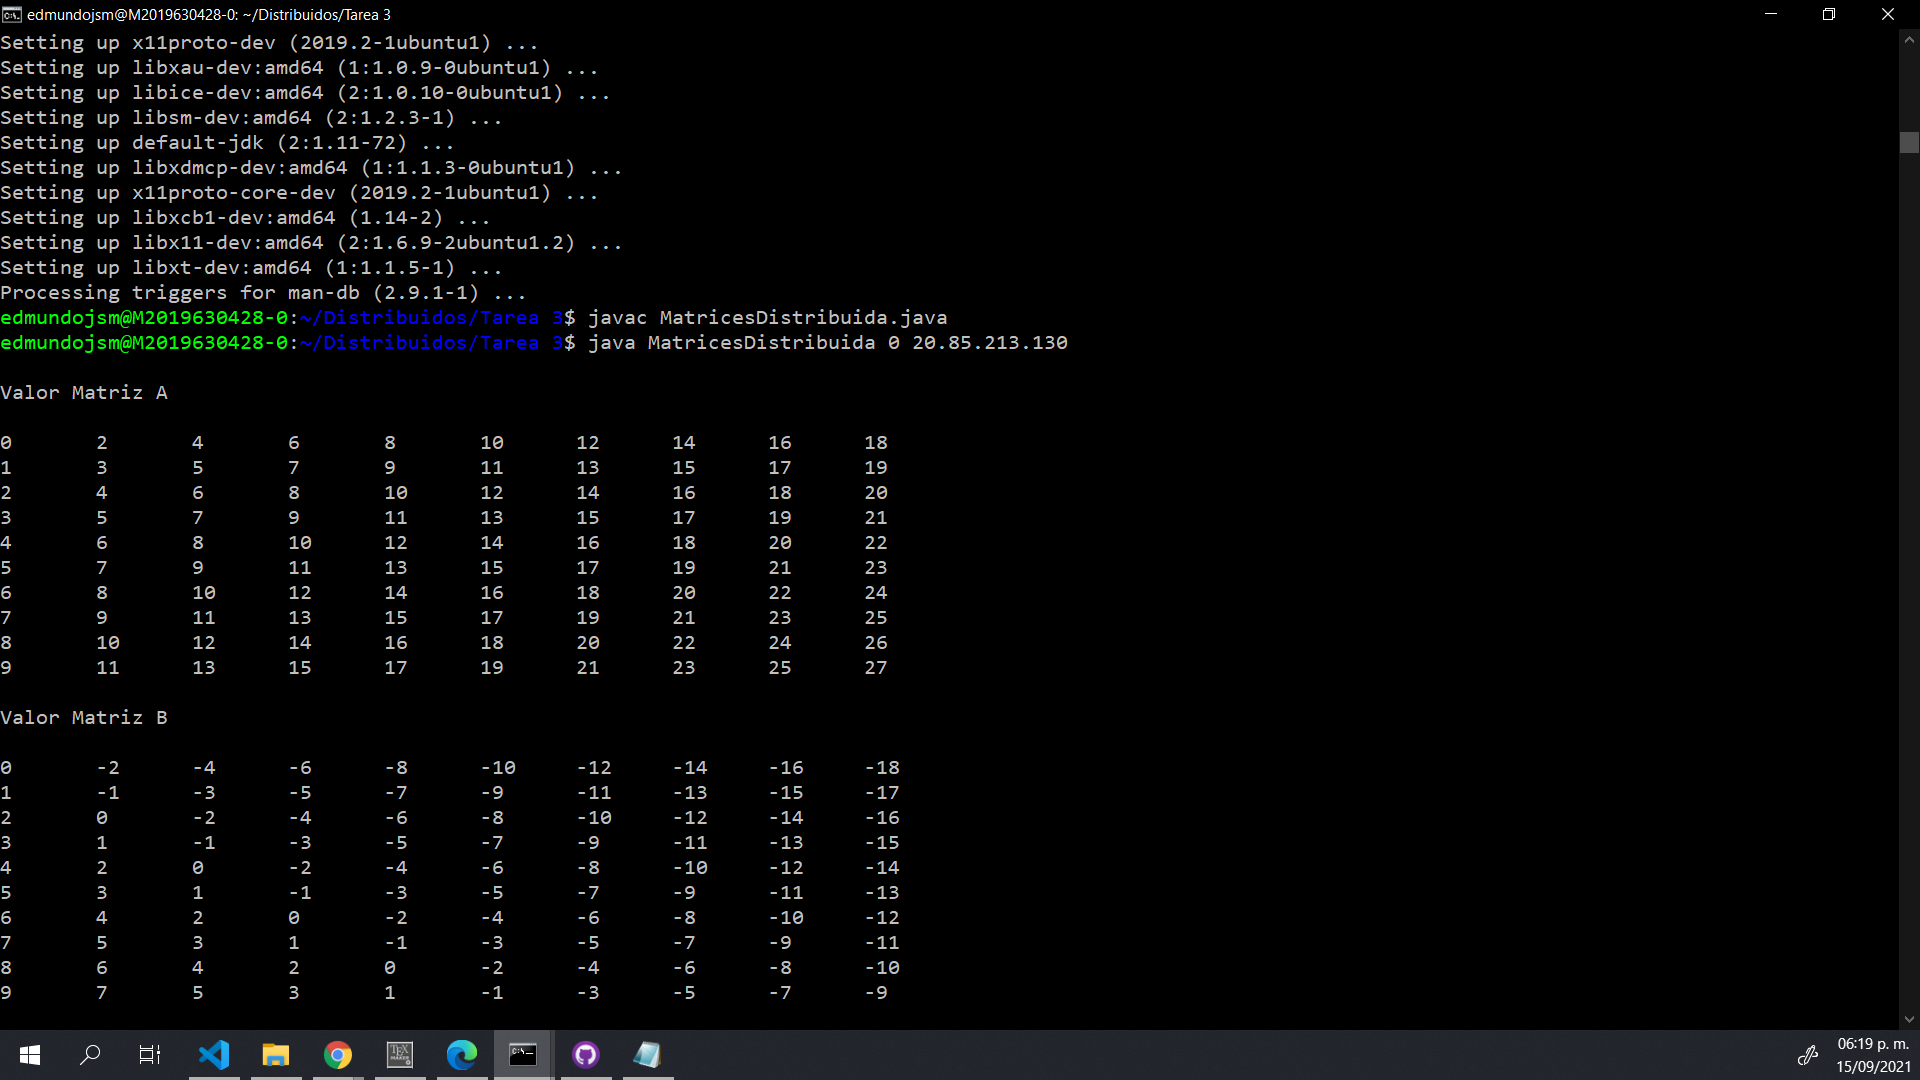
\includegraphics[scale=0.34]{resources/inicioNodo0.png}
			\caption{Compilación del código por medio de la terminal de Ubuntu de nuestra maquina virtual como nodo 0. }\label{fig:picture}
		\end{figure}
		\subsection{Ejecución del programa}
		\subsubsection{N=10}
		Una vez compilado nuestro programa en cada maquina virtual se procede a la ejecución de los nodos clientes como se ve en la figura 11 y del nodo servidor ver la figura 10.
		\begin{figure}[H]
			\centering
			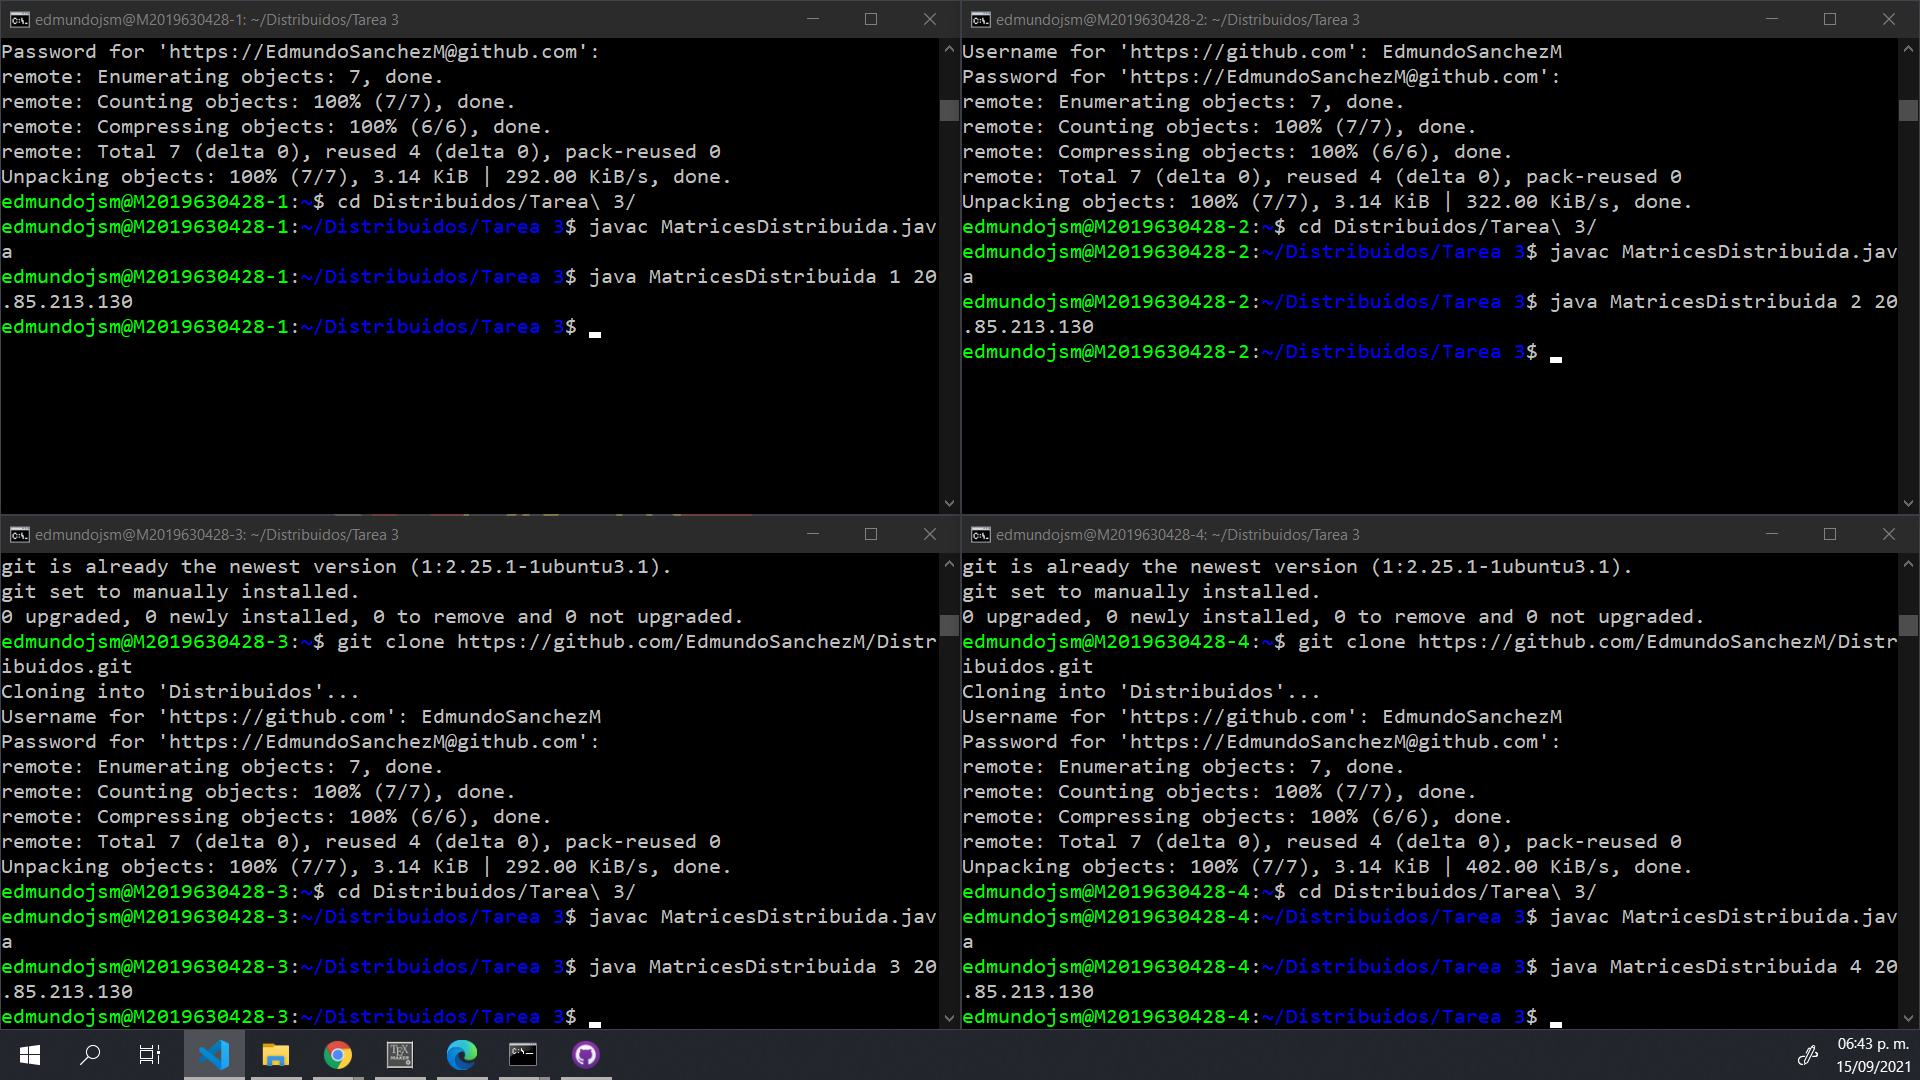
\includegraphics[scale=0.34]{resources/ejecucionnodo1a4n10.png}
			\caption{Ejecución del programa en los 4 nodos clientes. }\label{fig:picture}
		\end{figure}
		Al finalizar los 4 nodos clientes podemos ver como en el nodo servidor, es decir, el nodo 0 se despliega la matriz C y el valor de checksum de ésta (ver imagen 12 y 13).
		\begin{figure}[H]
			\centering
			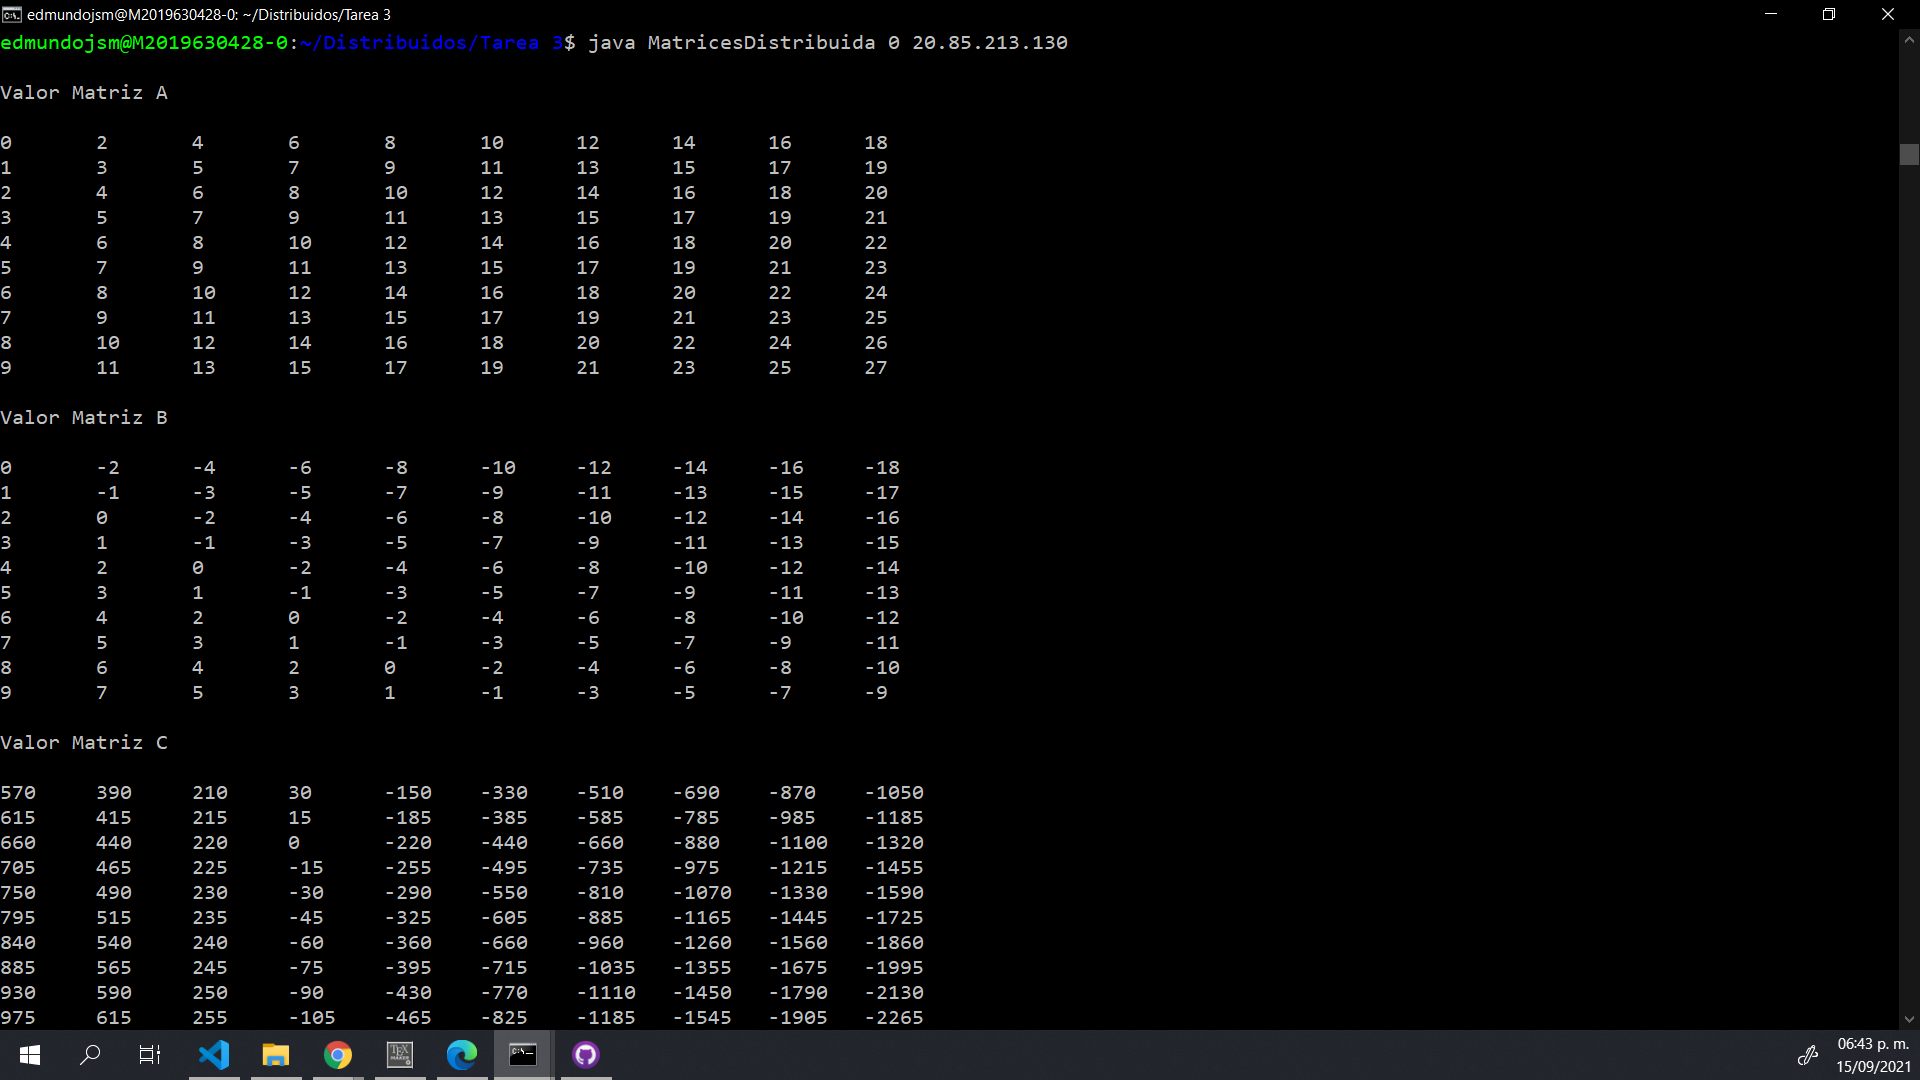
\includegraphics[scale=0.34]{resources/nodo0final1n10.png}
			\caption{Final de la ejecución del programa en el nodo 0. Parte 1.}\label{fig:picture}
		\end{figure}
		\begin{figure}[H]
			\centering
			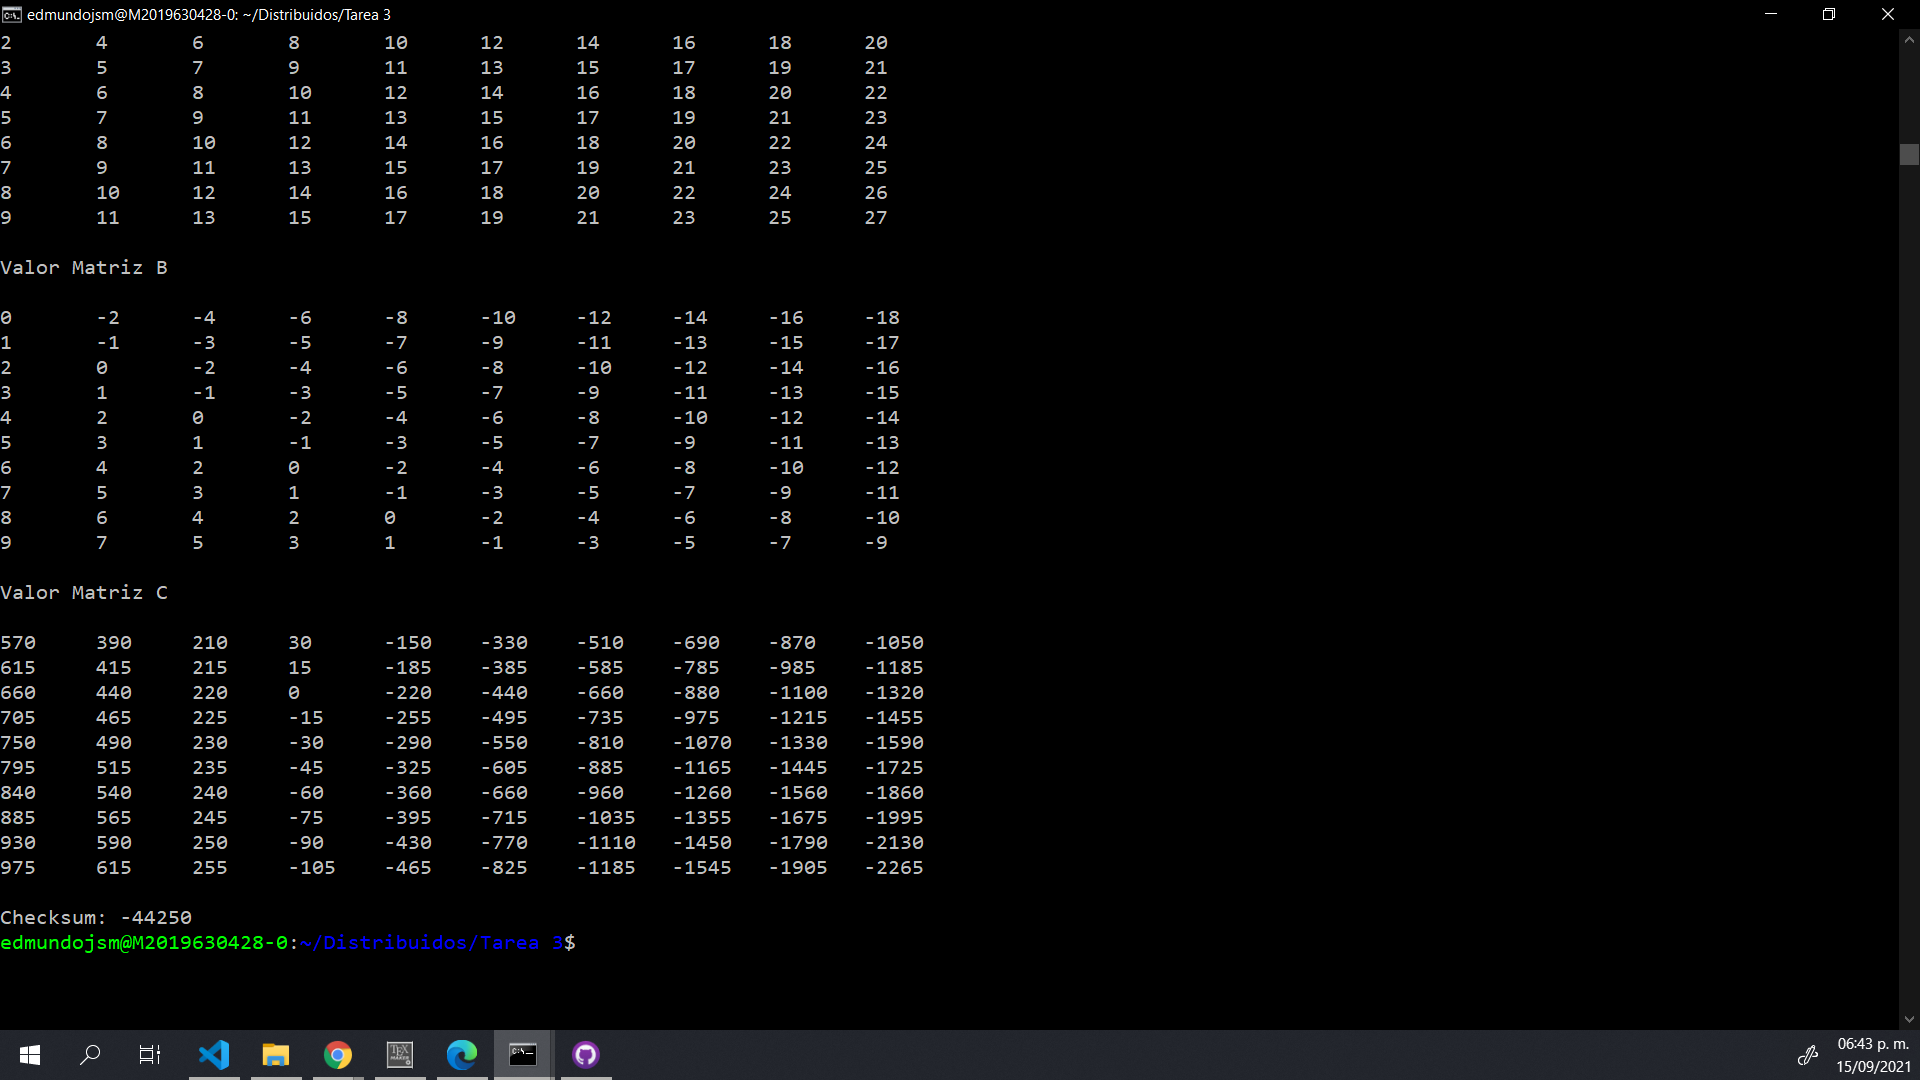
\includegraphics[scale=0.34]{resources/nodo0final2n10.png}
			\caption{Final de la ejecución del programa en el nodo 0. Parte 2.}\label{fig:picture}
		\end{figure}
		Como vemos se nos despliega el los valores de la matriz A, B y C así como el checksum de la matriz C, que es como se nos pide en la tarea. Veamos ahora el siguiente caso con N=1500.
		\subsubsection{N=1500}
		Para este caso se tuvo que modificar el programa asignando 1500 a la variable N, volver a subir el archivo a GitHub y usar el comando git pull para recibir las actualizaciones del repositorio, volver a compilar el archivo y ejecutarlo, todo lo anterior se puede ver en la figura 14.
		\begin{figure}[H]
			\centering
			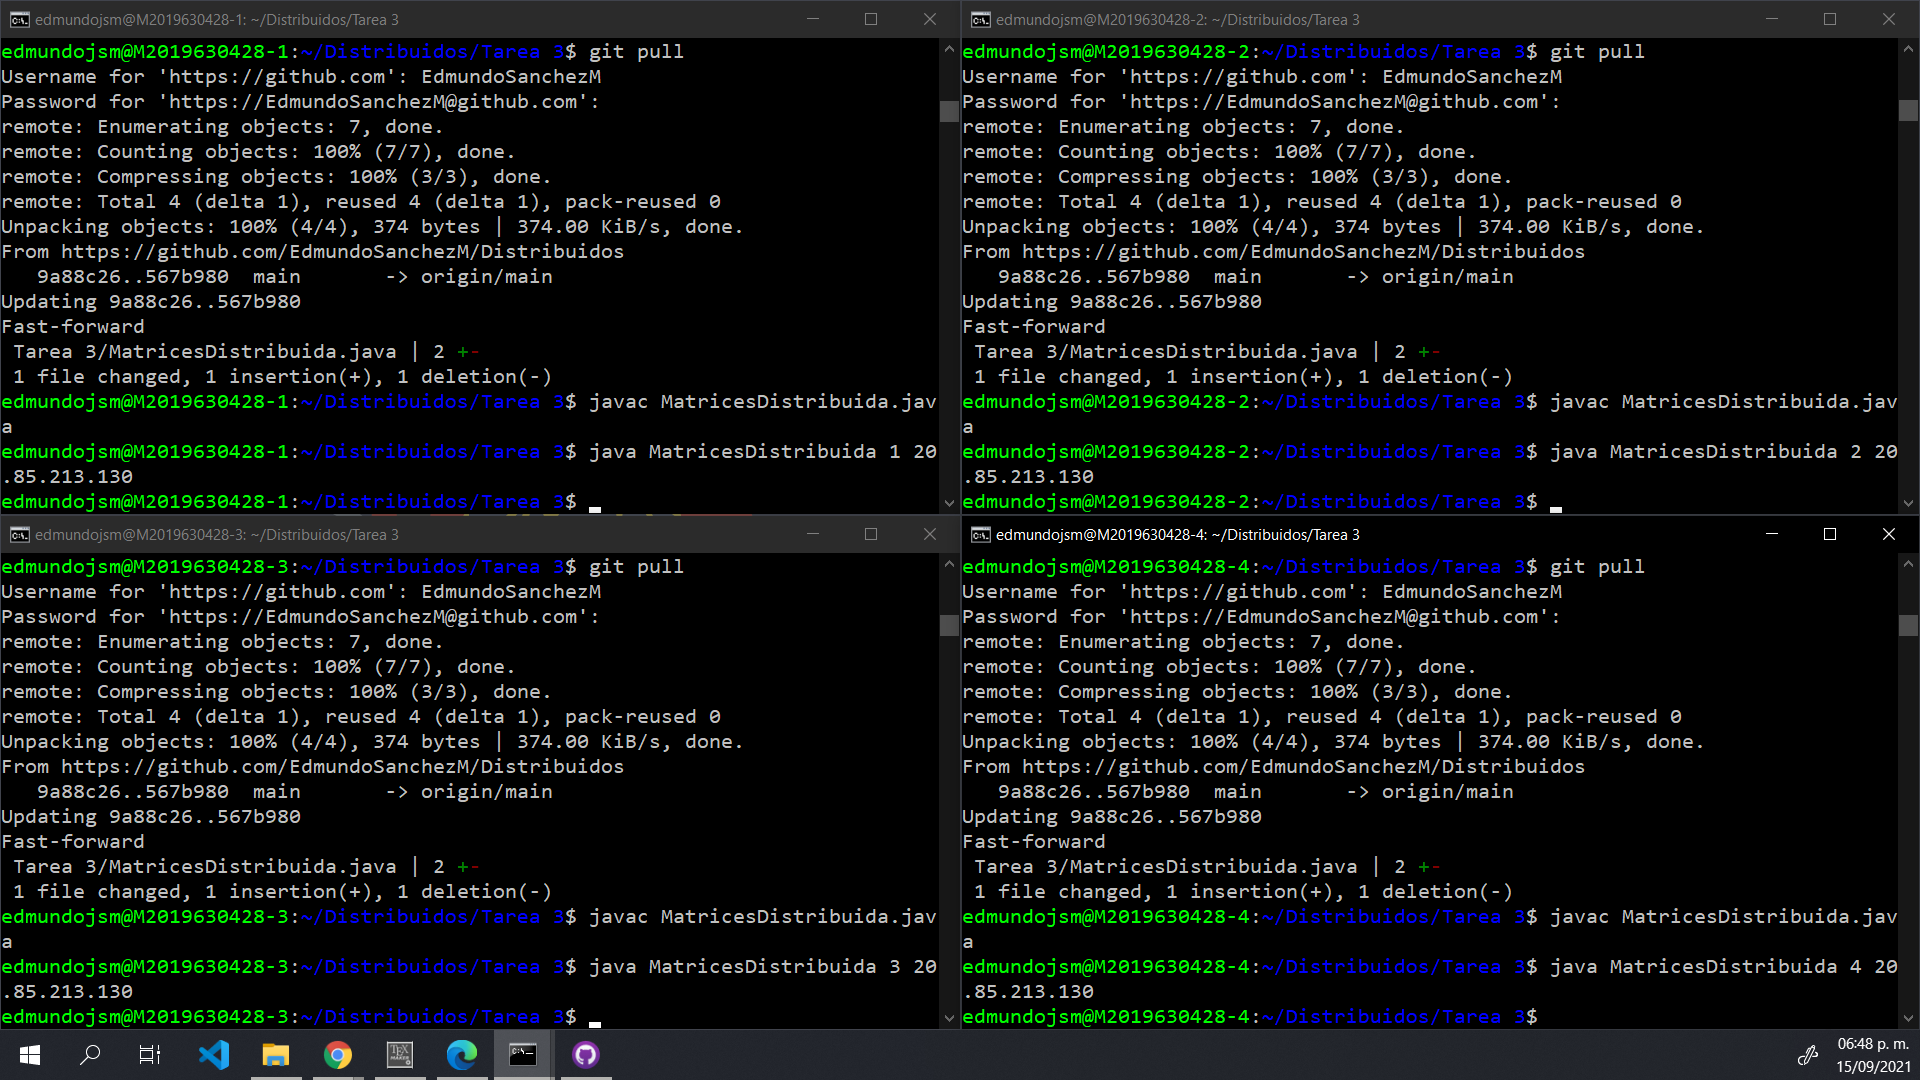
\includegraphics[scale=0.34]{resources/ejecucionnodo1a4n1500.png}
			\caption{Actualización, compilación y ejecución del programa en los 4 nodos clientes. }\label{fig:picture}
		\end{figure}
		Al finalizar los 4 nodos clientes podemos ver como en el nodo servidor, es decir, el nodo 0 solo se nos despliega el valor del checksum de la matriz C obtenida, al mismo tiempo podemos ver la actualización, compilación y ejecución de nuestro programa, todo esto se ve en la figura 15.
		\begin{figure}[H]
			\centering
			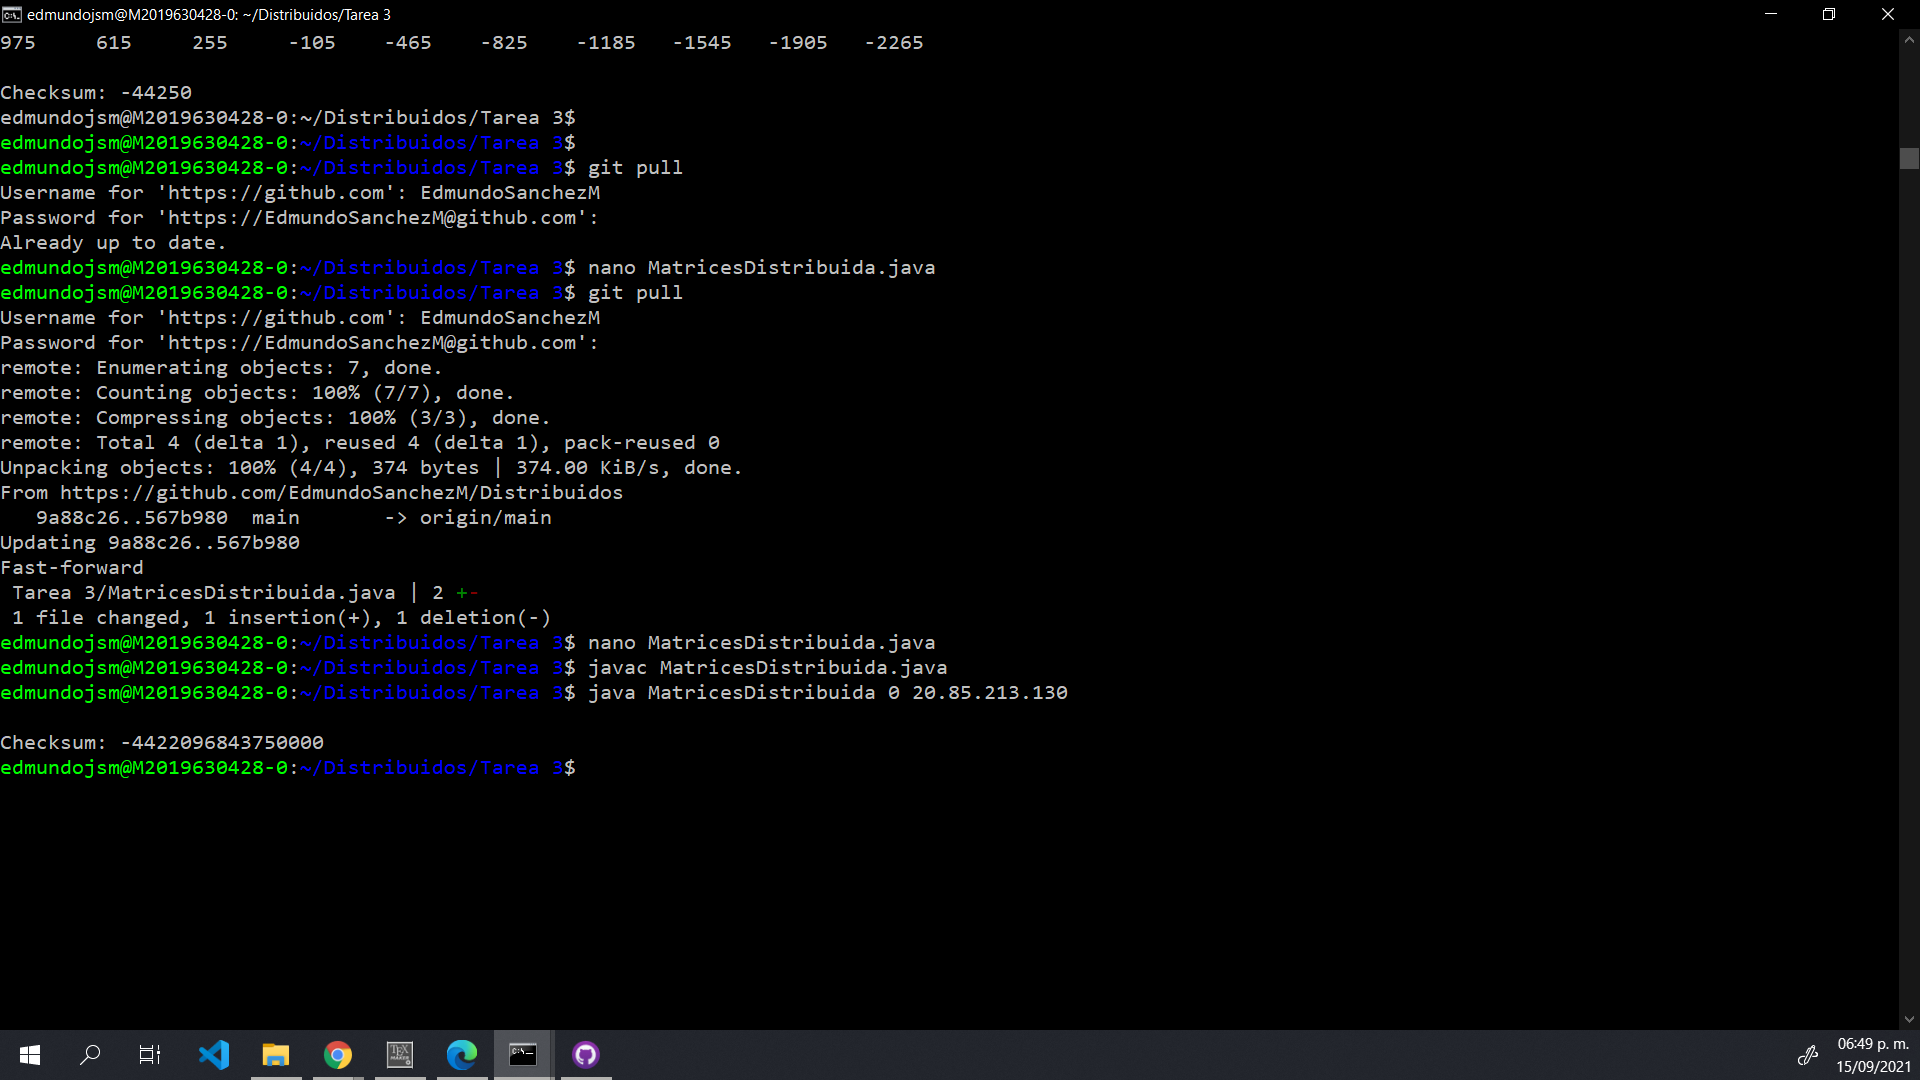
\includegraphics[scale=0.34]{resources/nodo0finaln1500.png}
			\caption{Final de la ejecución del programa en el nodo 0. Parte 1.}\label{fig:picture}
		\end{figure}
		Como vemos solo se nos despliega el valor del checksum de la matriz C, que es como se nos pide en la tarea.
		\subsection{Código}
	A continuación se anexa el código creado para el cumplimiento de esta tarea, notar que N es estático por lo que para probar diferentes casos de N necesitamos cambiar el valor de N en el programa y volver a compilar.
	\lstinputlisting[language = Java , frame = trBL , numbers=none]{../MatricesDistribuida.java}
	\section{Conclusiones}
	El desarrollo del código de la práctica fue muy interesante ya que es la primera vez en toda mi  instancia en ESCOM en la que uso una maquina virtual remota, en este caso de Azure y pude notar que es tener practica una maquina con Ubuntu pero sin interfaz gráfica y solo podemos usar los comandos que tiene Linux, ahora viendo la parte de la implementación de la practica no fue muy complicada ya que teníamos experiencia anterior con este tipo de topologia y requisitos, lo mas interesante sin duda de esta practica en mi opinión fueron dos cosas la primera el uso de maquinas virtuales remotas y la segunda fue el como enviar las partes de las matriz a los nodos, en mi caso mande numero a numero el contenido de las matrices, otra forma y la cual podría ser la mas simple seria mandar toda la parte de la matriz que se solicita como un objeto, sin embargo, considere que lo mejor seria mandar elemento a elemento del arreglo ya que considero que es mas eficiente.

\end{document}
